% !TEX TS-program = XeLaTeX
% !TEX encoding = UTF-8 Unicode

%%%%%%%%%%%%%%%%%%%%%%%%%%%%%%%%%%%%%%%%%%%%%%%%%%%%%%%%%%%%%%%%%%%%%%
%
%	大连理工大学博士论文 XeLaTeX 模版 —— 主文件 main.tex
% 版本:0.86
% 最后更新:2014.05.22
% 修改者:Yuri (E-mail: yuri_1985@163.com)
% 修订者:zzupc(E-mail: zzupchd@gmail.com;微博:http://weibo.com/zzupc)
% 编译环境1:Ubuntu 12.04 + TeXLive 2011 + Emacs
% 编译环境2:Windows 7 + CTeX v2.9.2.164 + WinEdit
%
%%%%%%%%%%%%%%%%%%%%%%%%%%%%%%%%%%%%%%%%%%%%%%%%%%%%%%%%%%%%%%%%%%%%%%

\documentclass[12pt, a4paper, openany, oneside, x11names]{book}
\usepackage{pdflscape}

% 字体配置文件
% !TEX TS-program = XeLaTeX
% !TEX encoding = UTF-8 Unicode

%%%%%%%%%%%%%%%%%%%%%%%%%%%%%%%%%%%%%%%%%%%%%%%%%%%%%%%%%%%%%%%%%%%%%% 
% 
% 大连理工大学硕士论文 XeLaTeX 模版 —— 字体配置文件 fonts.tex
% 版本:0.82
% 最后更新:2012.05.08
% 修改者:Yuri (E-mail: yuri_1985@163.com)
% 修订者:whufanwei(E-mail: dutfanwei@qq.com) 
% 编译环境1:Ubuntu 12.04 + TeXLive 2011 + Emacs
% 编译环境2:Windows 7 + CTeX v2.9.2.164 + WinEdit
% 
%%%%%%%%%%%%%%%%%%%%%%%%%%%%%%%%%%%%%%%%%%%%%%%%%%%%%%%%%%%%%%%%%%%%%% 

% 英文字体设置特别推荐方案(Windows,需要安装 Adobe 字体),现代
\usepackage{fontspec}
\usepackage{xltxtra,xunicode}
\usepackage[CJKnumber,CJKchecksingle,BoldFont]{xeCJK}
\usepackage{amsmath}
\usepackage{amssymb}
\setmainfont[Mapping=tex-text]{Times New Roman}
\setsansfont[Mapping=tex-text]{Arial} 
\setmonofont{Consolas}


% 英文字体设置方案一(Windows,需要安装 LM10 字体),和 LaTeX 默认字体保持一致,经典
% \usepackage{amssymb}
% \usepackage{fontspec}
% \usepackage{amsmath}
% \usepackage[CJKnumber,CJKaddspaces,CJKchecksingle,BoldFont]{xeCJK}
% \usepackage{mathrsfs}   % 一种常用于定义泛函算子的花体字母,只有大写。
% \usepackage{bm}         % 处理数学公式中的黑斜体的宏包
% \setmainfont{LMRoman10-Regular}
% \setsansfont{LMSans10-Regular}
% \setmonofont{LMMono10-Regular}

% 英文字体设置方案二(Linux,使用自带 LM10 字体),和 LaTeX 默认字体保持一致,经典
% \usepackage{fontspec}
% \usepackage{amsmath,amssymb}
% \usepackage[CJKnumber,CJKaddspaces,CJKchecksingle,BoldFont]{xeCJK}
% \usepackage{mathrsfs}   % 一种常用于定义泛函算子的花体字母,只有大写。
% \usepackage{bm}         % 处理数学公式中的黑斜体的宏包
% \setmainfont{LMRoman10}
% \setsansfont{LMSans10}
% \setmonofont{LMMono10}

% 英文字体设置方案三(Linux,使用自带 Nimbus 字体),和 Word 模版字体保持一致,经典
% \usepackage{fontspec}
% \usepackage{mathptmx}
% \usepackage{amsmath,amssymb}
% \usepackage[CJKnumber,CJKaddspaces,CJKchecksingle,BoldFont]{xeCJK}
% \usepackage{mathrsfs}   % 一种常用于定义泛函算子的花体字母,只有大写。
% \usepackage{bm}         % 处理数学公式中的黑斜体的宏包
% \setmainfont{Nimbus Roman No9 L}
% \setsansfont{Nimbus Sans L}
% \setmonofont{Nimbus Mono L}

% 中文字体设置,使用的是 Adobe 字体,保证了在 Adobe Reader / Acrobat 下优秀的显示效果
\setCJKmainfont[BoldFont={Adobe Heiti Std},ItalicFont={Adobe Kaiti Std}]{Adobe Song Std}
\setCJKsansfont{Adobe Heiti Std}
\setCJKmonofont{Adobe Fangsong Std}

% 定义字体名称,可在此添加自定义的字体
\setCJKfamilyfont{song}{Adobe Song Std}
\setCJKfamilyfont{hei}{Adobe Heiti Std}
\setCJKfamilyfont{kai}{Adobe Kaiti Std}
\setCJKfamilyfont{fs}{Adobe Fangsong Std}
\setCJKfamilyfont{xkai}{STXingkai}

% 自动调整中英文之间的空白
% \punctstyle{quanjiao}
\XeTeXlinebreaklocale "zh"      %中文断行
\XeTeXlinebreakskip = 0pt plus 1pt %1pt左右弹性间距
% 其他字体宏包



% 宏包配置文件
% !TEX TS-program = XeLaTeX
% !TEX encoding = UTF-8 Unicode

%%%%%%%%%%%%%%%%%%%%%%%%%%%%%%%%%%%%%%%%%%%%%%%%%%%%%%%%%%%%%%%%%%%%
%
% 大连理工大学硕士论文 XeLaTeX 模版 —— 宏包配置文件 packages.tex
% 版本:0.82
% 最后更新:2012.05.08
% 修改者:Yuri (E-mail: yuri_1985@163.com)
% 修订者:whufanwei(dutfanwei@qq.com)
% 编译环境1:Ubuntu 12.04 + TeXLive 2011 + Emacs
% 编译环境2:Windows 7 + CTeX v2.9.2.164 + WinEdit
%%%%%%%%%%%%%%%%%%%%%%%%%%%%%%%%%%%%%%%%%%%%%%%%%%%%%%%%%%%%%%%%%%%%%

% 页面设置
\usepackage[body={16.1cm, 22.2cm}]{geometry}
\usepackage{indentfirst}                         % 首行缩进宏包
\usepackage[sf]{titlesec}                        % 控制标题的宏包
\usepackage{titletoc}                            % 控制目录的宏包
\usepackage{fancyhdr}                            % 自定义页眉页脚
\usepackage{fancyref}                            % 引用链接属性
\usepackage[perpage,symbol]{footmisc}            % 脚注控制
\usepackage{layouts}                             % 打印当前页面格式的宏包
\usepackage{paralist}                            % 一种换行不缩进的列表格式,asparaenum,inparaenum 等
\usepackage[shortlabels]{enumitem}               % 列表格式
\usepackage{fancyvrb}                            % 原样输出
\usepackage[amsmath,thmmarks,hyperref]{ntheorem} % 定理类环境宏包
\usepackage{type1cm}                             % 控制字体的大小
\usepackage{enumitem}
\usepackage{pdfpages}
% 表格处理
\usepackage{booktabs}   % 三线表
\usepackage{multirow}   % 表格多行处理
\usepackage{diagbox}    % 斜线表头
\usepackage{tabularx}   % 表格折行
\usepackage{siunitx}    % 国际单位,小数点对齐

% 图形相关
\usepackage{graphicx}         % 请在引用图片时务必给出后缀名
\usepackage{xcolor} % 支持彩色
\usepackage[below]{placeins}  % 浮动图形控制宏包
\usepackage{rotating}	      % 图形和表格的控制
\usepackage{picinpar}
\usepackage{setspace}         % 定制表格和图形的多行标题行距
\usepackage{subfigure}           % 插入子图形
\usepackage[subfigure]{ccaption} % 插图表格的双语标题

\usepackage{listings}         % 源代码展示
\lstset{%
  language=TeX,
  defaultdialect=empty,
  basicstyle=\ttfamily\small,
  backgroundcolor=\color{LightSteelBlue1},
  keywordstyle=\color{blue},
  showspaces=false,
  showstringspaces=false,
  showtabs=false,
  tabsize=2,breakatwhitespace=false,
  columns=flexible}

% 其他
\usepackage{calc}   % 在 tex 文件中具有一些计算功能,主要用在页面控制。
\usepackage[xetex,
bookmarksnumbered=true,
bookmarksopen=true,
colorlinks=true,
% pdfborder={0 0 1},
citecolor=blue,
linkcolor=blue,
anchorcolor=green,
urlcolor=magenta,
breaklinks=true,
CJKbookmarks=true,
]{hyperref}


\usepackage[numbers,sort&compress,square,super]{natbib} %参考文献
\usepackage{hypernat}
\usepackage{bibentry}



\usepackage{rotating}
\usepackage{lscape}







% 格式文件
% !TEX TS-program = XeLaTeX
% !TEX encoding = UTF-8 Unicode

%%%%%%%%%%%%%%%%%%%%%%%%%%%%%%%%%%%%%%%%%%%%%%%%%%%%%%%%%%%%%%%%%%%%%%
%
%	大连理工大学博士论文 XeLaTeX 模版 —— 格式文件 format.tex
%	版本:0.71
%	最后更新:2010.12.22
%	修改者:Yuri (E-mail: yuri_1985@163.com)
%	编译环境:Ubuntu 10.04 + TeXLive 2010 + TeXworks
% Windows XP SP3 + CTeXLive 2009 + WinEdt 5.6
%
%%%%%%%%%%%%%%%%%%%%%%%%%%%%%%%%%%%%%%%%%%%%%%%%%%%%%%%%%%%%%%%%%%%%%%

%%%%%%%%%%%%%%%%%%%%%%%%%%%%%%%%%%%%%%%%%%%%%%%%%%%%%%%%%%%%%%%%%%%%%%
% 页面设置
%%%%%%%%%%%%%%%%%%%%%%%%%%%%%%%%%%%%%%%%%%%%%%%%%%%%%%%%%%%%%%%%%%%%%%
% A4 纸张
\setlength{\paperwidth}{21.0cm}
\setlength{\paperheight}{29.7cm}
% 设置正文尺寸大小
\setlength{\textwidth}{16.1cm}
\setlength{\textheight}{22.2cm}
% 设置正文区在正中间
\newlength \mymargin
\setlength{\mymargin}{(\paperwidth-\textwidth)/2}
%\setlength{\oddsidemargin}{(\mymargin)-1in}
%\setlength{\evensidemargin}{(\mymargin)-1in}
% 设置正文区偏移量,奇数页向右偏,偶数页向左偏
\newlength \myshift
\setlength{\myshift}{0.35cm}	% 双面打印的奇偶页偏移值,可根据需要修改,建议小于 0.5cm
%\addtolength{\oddsidemargin}{\myshift}
%\addtolength{\evensidemargin}{-\myshift}
% 页眉页脚相关距离设置
\setlength{\topmargin}{-0.05cm}
\setlength{\headheight}{0.50cm}
\setlength{\headsep}{0.90cm}
\setlength{\footskip}{1.47cm}
% 公式的精调
\allowdisplaybreaks[4]  % 可以让公式在排不下的时候分页排,这可避免页面有大段空白。

% 下面这组命令使浮动对象的缺省值稍微宽松一点,从而防止幅度
% 对象占据过多的文本页面,也可以防止在很大空白的浮动页上放置很小的图形。
\renewcommand{\topfraction}{0.9999999}
\renewcommand{\textfraction}{0.0000001}
\renewcommand{\floatpagefraction}{0.9999}

%%%%%%%%%%%%%%%%%%%%%%%%%%%%%%%%%%%%%%%%%%%%%%%%%%%%%%%%%%%%%%%%%%%%%%
% 字体字号定义
%%%%%%%%%%%%%%%%%%%%%%%%%%%%%%%%%%%%%%%%%%%%%%%%%%%%%%%%%%%%%%%%%%%%%%
% 字号
\newcommand{\yihao}{\fontsize{26pt}{39pt}\selectfont}	    % 一号,1.5  倍行距
\newcommand{\xiaoyi}{\fontsize{24pt}{30pt}\selectfont}      % 小一,1.25 倍行距
\newcommand{\erhao}{\fontsize{22pt}{27.5pt}\selectfont}     % 二号,1.25 倍行距
\newcommand{\xiaoer}{\fontsize{18pt}{22.5pt}\selectfont}    % 小二,1.25 倍行距
\newcommand{\sanhao}{\fontsize{16pt}{20pt}\selectfont}      % 三号,1.25 倍行距
\newcommand{\xiaosan}{\fontsize{15pt}{19pt}\selectfont}     % 小三,1.25 倍行距
\newcommand{\sihao}{\fontsize{14pt}{17.5pt}\selectfont}     % 四号,1.25倍行距
\newcommand{\daxiaosi}{\fontsize{12pt}{18pt}\selectfont}    % 小四,1.5 倍行距
\newcommand{\xiaosi}{\fontsize{12pt}{15pt}\selectfont}      % 小四,1.25倍行距
\newcommand{\dawu}{\fontsize{10.5pt}{18pt}\selectfont}      % 五号,1.75倍行距
\newcommand{\zhongwu}{\fontsize{10.5pt}{16pt}\selectfont}   % 五号,1.5 倍行距
\newcommand{\wuhao}{\fontsize{10.5pt}{10.5pt}\selectfont}   % 五号,单倍行距
\newcommand{\xiaowu}{\fontsize{9pt}{9pt}\selectfont}	    % 小五,单倍行距

\newcommand{\song}{\CJKfamily{song}}
\newcommand{\hei}{\CJKfamily{hei}}
\newcommand{\kai}{\CJKfamily{kai}}
\newcommand{\fs}{\CJKfamily{fs}}
\newcommand{\xkai}{\CJKfamily{xkai}}
\newcommand{\hwxh}{\CJKfamily{hwxh}}    % 华文细黑
\newfontfamily\Roman{Times New Roman}

% defaultfont 默认字体命令
\def\defaultfont{\renewcommand{\baselinestretch}{1.27}
  \fontsize{12pt}{15pt}\selectfont}

% 设置目录字体和行间距
\def\defaultmenufont{\renewcommand{\baselinestretch}{1.22}
  \fontsize{12pt}{15pt}\selectfont}

% 固定距离内容填入及下划线
\makeatletter
\newcommand\fixeddistanceleft[2][1cm]{{\hb@xt@ #1{#2\hss}}}
\newcommand\fixeddistancecenter[2][1cm]{{\hb@xt@ #1{\hss#2\hss}}}
\newcommand\fixeddistanceright[2][1cm]{{\hb@xt@ #1{\hss#2}}}
\newcommand\fixedunderlineleft[2][1cm]{\underline{\hb@xt@ #1{#2\hss}}}
\newcommand\fixedunderlinecenter[2][1cm]{\underline{\hb@xt@ #1{\hss#2\hss}}}
\newcommand\fixedunderlineright[2][1cm]{\underline{\hb@xt@ #1{\hss#2}}}
\makeatother

%%%%%%%%%%%%%%%%%%%%%%%%%%%%%%%%%%%%%%%%%%%%%%%%%%%%%%%%%%%%%%%%%%%%%%
% 标题环境相关
%%%%%%%%%%%%%%%%%%%%%%%%%%%%%%%%%%%%%%%%%%%%%%%%%%%%%%%%%%%%%%%%%%%%%%
% 定义、定理等环境
\theoremstyle{plain}
\theoremheaderfont{\hei\bf}
\theorembodyfont{\song\rmfamily}
\newtheorem{definition}{\hei 定义}[chapter]
\newtheorem{example}{\hei 例}[chapter]
\newtheorem{algorithm}{\hei 算法}[chapter]
\newtheorem{theorem}{\hei 定理}[chapter]
\newtheorem{axiom}{\hei 公理}[chapter]
\newtheorem{proposition}[theorem]{\hei 命题}
\newtheorem{property}{\hei 性质}
\newtheorem{lemma}[theorem]{\hei 引理}
\newtheorem{corollary}{\hei 推论}[chapter]
\newtheorem{remark}{\hei 注解}[chapter]
\newenvironment{proof}{\hei{证明} }{\hfill $\square$ \vskip 4mm}
\newtheorem{method}{\hei 方法}[chapter]
% 目录标题
\renewcommand\contentsname{\hfill 目  录 \hfill}
\renewcommand\listfigurename{\hfill 图~目~录 \hfill}
\renewcommand\listtablename{\hfill 表~目~录 \hfill}
\renewcommand{\bibname}{\hfill 参~考~文~献 \hfill}

% 自定义项目列表标签及格式 \begin{publist} 列表项 \end{publist}
\newcounter{pubctr} %自定义新计数器
\newenvironment{publist}{%%%%%定义新环境
\begin{list}{[\arabic{pubctr}]} %%标签格式
    {
     \usecounter{pubctr}
     \setlength{\leftmargin}{2.5em}     % 左边界 \leftmargin =\itemindent + \labelwidth + \labelsep
     \setlength{\itemindent}{0em}     % 标号缩进量
     \setlength{\labelsep}{1em}       % 标号和列表项之间的距离,默认0.5em
     \setlength{\rightmargin}{0em}    % 右边界
     \setlength{\topsep}{0ex}         % 列表到上下文的垂直距离
     \setlength{\parsep}{0ex}         % 段落间距
     \setlength{\itemsep}{0ex}        % 标签间距
     \setlength{\listparindent}{0pt} % 段落缩进量
    }}
{\end{list}}%%%%%


%%%%%%%%%%%%%%%%%%%%%%%%%%%%%%%%%%%%%%%%%%%%%%%%%%%%%%%%%%%%%%%%%%%%%%
% 段落章节相关
%%%%%%%%%%%%%%%%%%%%%%%%%%%%%%%%%%%%%%%%%%%%%%%%%%%%%%%%%%%%%%%%%%%%%%
\setcounter{secnumdepth}{4}
\setcounter{tocdepth}{4}
% 设置章、节、小节、小小节的间距
\titleformat{\chapter}[hang]{\normalfont\xiaosan\hei\sf}{\xiaosan\thechapter}{1em}{\xiaosan}
\titlespacing{\chapter}{0pt}{-3ex  plus .1ex minus .2ex}{3.3ex}
\titleformat{\section}[hang]{\sihao\hei\sf}{\sihao\thesection}{1em}{}{}
\titlespacing{\section}{0pt}{0.5em}{0.5em}
\titleformat{\subsection}[hang]{\xiaosi\hei\sf}{\xiaosi\thesubsection}{1em}{}{}
\titlespacing{\subsection}{0pt}{0.5em}{0.3em}
\titleformat{\subsubsection}[hang]{\hei\sf}{\thesubsubsection}{1em}{}{}
\titlespacing{\subsubsection}{0pt}{0.3em}{0pt}
% 缩小目录中各级标题之间的缩进
\dottedcontents{chapter}[0.32cm]{\vspace{0.2em}}{1.0em}{5pt}
\dottedcontents{section}[1.32cm]{}{1.8em}{5pt}
\dottedcontents{subsection}[2.32cm]{}{2.7em}{5pt}
\dottedcontents{subsubsection}[3.32cm]{}{3.4em}{5pt}

% 段落之间的竖直距离
\setlength{\parskip}{1.2pt}
% 段落缩进
\setlength{\parindent}{24pt}
% 定义行距
\renewcommand{\baselinestretch}{1.27}
% 参考文献条目间行间距
\setlength{\bibsep}{2pt}

%%%%%%%%%%%%%%%%%%%%%%%%%%%%%%%%%%%%%%%%%%%%%%%%%%%%%%%%%%%%%%%%%%%%%%
% 页眉页脚设置
%%%%%%%%%%%%%%%%%%%%%%%%%%%%%%%%%%%%%%%%%%%%%%%%%%%%%%%%%%%%%%%%%%%%%%

\newcommand{\makeheadrule}{%
  \makebox[0pt][l]{\rule[.7\baselineskip]{\headwidth}{0.5pt}}%
  \vskip-.8\baselineskip}

\makeatletter
\renewcommand{\headrule}{%
  {\if@fancyplain\let\headrulewidth\plainheadrulewidth\fi
    \makeheadrule}}

\pagestyle{fancyplain}

\fancyhf{}
\fancyhead[CO]{\song\wuhao{大连理工本科学士论文模版}}
%\fancyhead[CE]{\song\wuhao\@ctitle}
\fancyfoot[C,C]{\xiaowu$-$~\thepage~$-$}

% Clear Header Style on the Last Empty Odd pages
\makeatletter
\def\cleardoublepage{\clearpage\if@twoside \ifodd\c@page\else%
  \hbox{}%
  \thispagestyle{empty}%              % Empty header styles
  \newpage%
  \if@twocolumn\hbox{}\newpage\fi\fi\fi}


\def\engcontentsname{CONTENTS}
\renewcommand\engcontentsname{\normalfont \hfill TABLE OF CONTENTS \hfill}
\newcommand\tableofengcontents{

     \@restonecolfalse
   \chapter*{\engcontentsname  %chapter*上移一行,避免在toc中出现。
       \@mkboth{%
          \engcontentsname}{\engcontentsname}}
   \@starttoc{toe}%
   \if@restonecol\twocolumn\fi
   }

%重新定义BiChapter命令,可实现标题手动换行,但不影响目录
\def\BiChapter{\relax\@ifnextchar [{\@BiChapter}{\@@BiChapter}}
\def\@BiChapter[#1]#2#3{\chapter[#1]{#2}
    \addcontentsline{toe}{chapter}{\xiaosi \thechapter\hspace{0.5em} #3}}
\def\@@BiChapter#1#2{\chapter{#1}
    \addcontentsline{toe}{chapter}{\xiaosi  \thechapter\hspace{0.5em}{\boldmath #2}}}

\newcommand{\BiSection}[2]
{   \section{#1}
    \addcontentsline{toe}{section}{\protect\numberline{\csname thesection\endcsname}#2}
}

\newcommand{\BiSubsection}[2]
{    \subsection{#1}
    \addcontentsline{toe}{subsection}{\protect\numberline{\csname thesubsection\endcsname}#2}
}

\newcommand{\BiSubsubsection}[2]
{    \subsubsection{#1}
    \addcontentsline{toe}{subsubsection}{\protect\numberline{\csname thesubsubsection\endcsname}#2}
}

\newcommand{\BiAppendixChapter}[2] % 该附录命令适用于发表文章,简历等
{\phantomsection
\markboth{#1}{#1}
\addcontentsline{toc}{chapter}{\xiaosi #1}
\addcontentsline{toe}{chapter}{\xiaosi #2}  \chapter*{#1}
}

\newcommand{\BiAppChapter}[2]    % 该附录命令适用于有章节的完整附录
{\phantomsection
 \chapter{#1}
 \addcontentsline{toe}{chapter}{\xiaosi Appendix \thechapter~~#2}
}

%%%%%%%%%%%%%%%%%%%%%%%%%%%%%%%%%%%%%%%%%%%%%%%%%%%%%%%%%%%%%%%%%%%%%%
% 列表环境设置

%%%%%%%%%%%%%%%%%%%%%%%%%%%%%%%%%%%%%%%%%%%%%%%%%%%%%%%%%%%%%%%%%%%%%%

\setlist[enumerate]{1、,itemsep=-5pt,topsep=0mm,labelindent=\parindent,leftmargin=*}
% \setlist[enumerate]{(1),itemsep=-5pt,topsep=0mm,labelindent=\parindent,leftmargin=*}模板有更新,换为1、

%%%%%%%%%%%%%%%%%%%%%%%%%%%%%%%%%%%%%%%%%%%%%%%%%%%%%%%%%%%%%%%%%%%%%%
% 国际单位,以点连接。
%%%%%%%%%%%%%%%%%%%%%%%%%%%%%%%%%%%%%%%%%%%%%%%%%%%%%%%%%%%%%%%%%%%%%%
\sisetup{inter-unit-product = { }\cdot{ }}

%%%%%%%%%%%%%%%%%%%%%%%%%%%%%%%%%%%%%%%%%%%%%%%%%%%%%%%%%%%%%%%%%%%%%%
% 参考文献的处理
%%%%%%%%%%%%%%%%%%%%%%%%%%%%%%%%%%%%%%%%%%%%%%%%%%%%%%%%%%%%%%%%%%%%%%

% \addtolength{\bibsep}{-0.5em}              % 缩小参考文献间的垂直间距
\setlength{\bibhang}{2em}
\bibpunct{[}{]}{,}{s}{}{}




% \let\orig@Itemize =\itemize
% \let\orig@Enumerate =\enumerate
% \let\orig@Description =\description

% \def\Myspacing{\itemsep=1ex \topsep=-4ex \partopsep=-2ex \parskip=-1ex \parsep=2ex}
% \def\newitemsep{
% \renewenvironment{itemize}{\orig@Itemize\Myspacing}{\endlist}
% \renewenvironment{enumerate}{\orig@Enumerate\Myspacing}{\endlist}
% \renewenvironment{description}{\orig@Description\Myspacing}{\endlist}
% }
%   \def\olditemsep{
%   \renewenvironment{itemize}{\orig@Itemize}{\endlist}
%   \renewenvironment{enumerate}{\orig@Enumerate}{\endlist}
%   \renewenvironment{description}{\orig@Description}{\endlist}
% }
%   \renewcommand{\labelenumi}{(\arabic{enumi})}
%   \newitemsep

%%%%%%%%%%%%%%%%%%%%%%%%%%%%%%%%%%%%%%%%%%%%%%%%%%%%%%%%%%%%%%%%%%%%%%
%   其他设置
%%%%%%%%%%%%%%%%%%%%%%%%%%%%%%%%%%%%%%%%%%%%%%%%%%%%%%%%%%%%%%%%%%%%%%
%   增加 \ucite 命令使显示的引用为上标形式
%   \newcommand{\ucite}[1]{$^{\mbox{\scriptsize \cite{#1}}}$}
\newcommand{\ucite}[1]{\scalebox{1.3}[1.3]{\raisebox{-0.65ex}{\cite{#1}}}}
%%%%%%%%%%%%%%%%%%%%%%%%%%%%%%%%%%%%%%%%%%%%%%%%%%%%%%%%%%%%%%%%%%%%%%
%   图形表格
%%%%%%%%%%%%%%%%%%%%%%%%%%%%%%%%%%%%%%%%%%%%%%%%%%%%%%%%%%%%%%%%%%%%%%
\renewcommand{\figurename}{图}
\renewcommand{\tablename}{表}
%\renewcommand{\thetable}{\thechapter-\arabic{table}} %修改表格的表头为表2-1

\renewcommand\listoftables{\vskip0.5cm
     %\par{\Large\bfseries \listtablename}\vskip1cm
     \section*{\listtablename}\vskip0.5cm
      \@mkboth{%
           \MakeUppercase\listtablename}%
          {\MakeUppercase\listtablename}%
     \@starttoc{lot}%
     }

\newcommand*{\noaddvspace}{\renewcommand*{\addvspace}[1]{}}
\addtocontents{lof}{\protect\noaddvspace}
\addtocontents{lot}{\protect\noaddvspace}


 \captionstyle{\centering}
 \hangcaption
\captiondelim{\hspace{1em}}
\captiondelim{\hspace{1em}}
%\captionnamefont{\song \xiaosi}%字体改为黑体
%\captiontitlefont{\song \xiaosi}
\captionnamefont{\song \zhongwu}%字体改为黑体小四
\captiontitlefont{\song \zhongwu}
\setlength{\abovecaptionskip}{0pt}
\setlength{\belowcaptionskip}{0pt}



\newcommand{\tablepage}[2]{\begin{minipage}{#1}\vspace{0.5ex} #2 \vspace{0.5ex}\end{minipage}}
\newcommand{\returnpage}[2]{\begin{minipage}{#1}\vspace{0.5ex} #2 \vspace{-1.5ex}\end{minipage}}


%%%%%%%%%%%%%%%%%%%%%%%%%%%%%%%%%%%%%%%%%%%%%%%%%%%%%%%%%%%%%%%%%%%%%%
% 定义题头格言的格式
%%%%%%%%%%%%%%%%%%%%%%%%%%%%%%%%%%%%%%%%%%%%%%%%%%%%%%%%%%%%%%%%%%%%%%

\newsavebox{\AphorismAuthor}
\newenvironment{Aphorism}[1]
{\vspace{0.5cm}\begin{sloppypar} \slshape
    \sbox{\AphorismAuthor}{#1}
    \begin{quote}\small\itshape }
    {\\ \hspace*{\fill}------\hspace{0.2cm} \usebox{\AphorismAuthor}
    \end{quote}
  \end{sloppypar}\vspace{0.5cm}}

% 自定义一个空命令,用于注释掉文本中不需要的部分。
\newcommand{\comment}[1]{}

% This is the flag for longer version
\newcommand{\longer}[2]{#1}

\newcommand{\ds}{\displaystyle}

% define graph scale
\def\gs{1.0}

%%%%%%%%%%%%%%%%%%%%%%%%%%%%%%%%%%%%%%%%%%%%%%%%%%%%%%%%%%%%%%%%%%%%%%%%%%%%%%%%
% 封面摘要
%%%%%%%%%%%%%%%%%%%%%%%%%%%%%%%%%%%%%%%%%%%%%%%%%%%%%%%%%%%%%%%%%%%%%%%%%%%%%%%%
\def\cdegree#1{\def\@cdegree{#1}}\def\@cdegree{}
\def\ctitle#1{\def\@ctitle{#1}}\def\@ctitle{}
\def\caffil#1{\def\@caffil{#1}}\def\@caffil{}
\def\csubject#1{\def\@csubject{#1}}\def\@csubject{}
\def\cschool#1{\def\@cschool{#1}}\def\@cschool{}
\def\cauthor#1{\def\@cauthor{#1}}\def\@cauthor{}
\def\cauthorno#1{\def\@cauthorno{#1}}\def\@cauthorno{}
\def\csupervisor#1{\def\@csupervisor{#1}}\def\@csupervisor{}
\def\creviewer#1{\def\@creviewer{#1}}\def\@creviewer{}
\def\cdate#1{\def\@cdate{#1}}\def\@cdate{}
\long\def\cabstract#1{\long\def\@cabstract{#1}}\long\def\@cabstract{}
\def\ckeywords#1{\def\@ckeywords{#1}}\def\@ckeywords{}
\def\etitle#1{\def\@etitle{#1}}\def\@etitle{}
\long\def\eabstract#1{\long\def\@eabstract{#1}}\long\def\@eabstract{}
\def\ekeywords#1{\def\@ekeywords{#1}}\def\@ekeywords{}

% 封面
\def\makecover{
  \begin{titlepage}
    \newpage
    \thispagestyle{empty}
    \begin{center}
      \parbox[t][4.40cm][c]{\textwidth}
      {
        \begin{center}
         	{\xiaoyi\song\textbf{\@cdegree}\\}
                    \vspace{1.36cm}
                   {\erhao\hwxh\bf{\@ctitle}\\}
                    \vspace{0.17cm}
                   {\sanhao\textbf{\@etitle}\\}
        \end{center}
      }
      \parbox[b][10.39cm][c]{\textwidth}
      {
        \vspace{8.2cm}
        \begin{center}
          {
            \xiaosan\song
            \begin{tabular}{p{0.6cm}p{6.7em}@{\extracolsep{0.4em}}lc}
              \vspace{-0.41cm}
              ~ & 学\hfill 院 (系):& \fixedunderlineleft[6.08cm]{\@cschool} & \\
              \vspace{-0.41cm}
              ~ & 专 \hfill 业:& \fixedunderlineleft[6.08cm]{\@csubject} & \\
              \vspace{-0.41cm}
              ~ & 学 \hfill 生 \hfill 姓 \hfill 名:& \fixedunderlineleft[6.08cm]{\@cauthor} & \\
              \vspace{-0.41cm}
              ~ & 学 \hfill 号:& \fixedunderlineleft[6.08cm]{\@cauthorno} & \\
              \vspace{-0.41cm}
              ~ & 指 \hfill 导 \hfill 教 \hfill 师:& \fixedunderlineleft[6.08cm]{\@csupervisor} & \\
              \vspace{-0.41cm}
              ~ & 评 \hfill 阅 \hfill 教 \hfill 师:& \fixedunderlineleft[6.08cm]{\@\creviewer} & \\
              \vspace{-0.41cm}
               ~ & 完 \hfill 成 \hfill 日 \hfill 期:& \fixedunderlineleft[6.08cm]{\@cdate} & \\
              \vspace{-0.41cm}
            \end{tabular}
          }
        \end{center}
      }

      \vspace{4.88cm}

      {
      	
     	\xiaoer\xkai
        大连理工大学\\
        %\vspace{0.24cm}
        \vspace{0.35cm}
        \xiaosi\song
        Dalian University of Technology
      }
    \end{center}
    \cleardoublepage
  \end{titlepage}
}

% 独创性说明
\def\originality{
  \renewcommand{\baselinestretch}{1.61}
  \newpage
  \thispagestyle{empty}
  \begin{center}
    \parbox[t][1.52cm][c]{\textwidth}
    {\xiaoer\song\centerline{大连理工大学学位论文独创性声明}}
    \parbox[t][7.68cm][c]{\textwidth}
    {
      \sihao\fs\noindent
        作者郑重声明:所呈交的学位论文,是本人在导师的指导下进行研究工作所取得的成果。%
      尽我所知,除文中已经注明引用内容和致谢的地方外,%
      本论文不包含其他个人或集体已经发表的研究成果,%
      也不包含其他已申请学位或其他用途使用过的成果。%
      与我一同工作的同志对本研究所做的贡献均已在论文中做了明确的说明并表示了谢意。%

      \vspace{0.47cm}\noindent
        若有不实之处,本人愿意承担相关法律责任。
    }
    \parbox[t][0.58cm][c]{\textwidth}
    {\sihao\fs 学{\hfill}位{\hfill}论{\hfill}文{\hfill}题{\hfill}目{\hfill}:\fixedunderlinecenter[12.6cm]{\@ctitle}}
    \parbox[t][1.22cm][c]{\textwidth}
    {\sihao\fs 作{\hfill}者{\hfill}签{\hfill}名{\hfill}:\fixeddistanceleft[12.6cm]{\underline{\hspace{5.8cm}}\hfill
	日期:\underline{\hspace{1.4cm}}~年~{\underline{\hspace{0.7cm}}~月~{\underline{\hspace{0.7cm}}~日~}}}}
  \end{center}
  \renewcommand{\baselinestretch}{1.27}
  \cleardoublepage
}

\def\authorization
{
\pagestyle{fancy}
\fancyfoot{}
  \begin{center}
    \sanhao\hei~大连理工大学学位论文版权使用授权书~
  \end{center}

  \sihao\fs\noindent
    本人完全了解学校有关学位论文知识产权的规定,%
  在校攻读学位期间论文工作的知识产权属于大连理工大学,允许论文被查阅和借阅。%
  学校有权保留论文并向国家有关部门或机构送交论文的复印件和电子版,%
  可以将本学位论文的全部或部分内容编入有关数据库进行检索,%
  可以采用影印、缩印、或扫描等复制手段保存和汇编本学位论文。%
  \\

  \vspace{0.2cm}\noindent
  学{\hfill}位{\hfill}论{\hfill}文{\hfill}题{\hfill}目{\hfill}:\fixedunderlinecenter[12.6cm]{\@ctitle}\\
  作{\hfill}者{\hfill}签{\hfill}名{\hfill}:\fixeddistanceleft[12.6cm]{\underline{\hspace{5.8cm}}\hfill
    日期:\underline{\hspace{1.4cm}}~年~{\underline{\hspace{0.7cm}}~月~{\underline{\hspace{0.7cm}}~日~}}}\\
  导{\hfill}师{\hfill}签{\hfill}名{\hfill}:\fixeddistanceleft[12.6cm]{\underline{\hspace{5.8cm}}\hfill
    日期:\underline{\hspace{1.4cm}}~年~{\underline{\hspace{0.7cm}}~月~{\underline{\hspace{0.7cm}}~日~}}}\\
  \renewcommand{\baselinestretch}{1.27}
}

\def\makeabstract{
  \defaultfont
  \chapter*{\hfill 摘  要 \hfill}
  \addcontentsline{toc}{chapter}{摘  要}
  \setcounter{page}{1}
  \@cabstract
  \vspace{0.53cm}

   {\hei{关键词:{\fs\@ckeywords}}}

  \defaultfont
  \cleardoublepage
  \chapter*{}
  \addcontentsline{toc}{chapter}{Abstract}
  \addcontentsline{toe}{chapter}{Abstract}
  \vspace{-1.40cm}
  \begin{center}
    {\xiaosan\textrm{\@etitle}}
  \end{center}
  \vspace{-0.35cm}
  \begin{center}
    {
      \xiaosan{Abstract}\\
    }
  \end{center}
  \vspace{0.12cm}

  \@eabstract

  \vspace{0.55cm}
   %\noindent {\textbf{Key Words:}}~~{\textsf{\@ekeywords}}%新论文模板将字体改为times new roman
   {\textbf{Key Words:}}~~{{\@ekeywords}}
  \cleardoublepage
}

\makeatletter
\def\hlinewd#1{%
  \noalign{\ifnum0=`}\fi\hrule \@height #1 \futurelet
  \reserved@a\@xhline}
\makeatother

% 定义索引生成
\def\generateindex
{
  \addcontentsline{toc}{chapter}{\indexname}
  \printindex
  \cleardoublepage
}

\raggedbottom





\begin{document}
\lstset{
backgroundcolor=\color{white},
basicstyle=\Roman\xiaosi, 
numberstyle=\Roman\xiaosi
}
% 定义所有的图片文件在 figures 子目录下
\graphicspath{{figures/}}

% 前言
\frontmatter
\pagenumbering{Roman}
% !TEX TS-program = XeLaTeX
% !TEX encoding = UTF-8 Unicode

%%%%%%%%%%%%%%%%%%%%%%%%%%%%%%%%%%%%%%%%%%%%%%%%%%%%%%%%%%%%%%%%%%%%%%
%
%	大连理工大学博士论文 XeLaTeX 模版 —— 封面文件 cover.tex
%	版本:0.71
%	最后更新:2010.12.22
%	修改者:Yuri (E-mail: yuri_1985@163.com)
%	编译环境:Ubuntu 10.04 + TeXLive 2010 + TeXworks
%             Windows XP SP3 + CTeXLive 2009 + WinEdt 5.6
%
%%%%%%%%%%%%%%%%%%%%%%%%%%%%%%%%%%%%%%%%%%%%%%%%%%%%%%%%%%%%%%%%%%%%%%

\cdegree{大连理工大学本科毕业设计(论文)}
\ctitle{大连理工大学本科学位论文~\XeLaTeX{}~模版}
\etitle{The \XeLaTeX{} Template of Bachelor Degree Thesis  of DUT}

% 根据需要添加字符间距
\cschool{{\quad\;}XXXXX学部}
\csubject{{\quad\;}专~~业}
\cauthor{{\quad\;}张~~ ~~三}
\cauthorno{{\quad\;}201281000}
\csupervisor{{\quad\;}王~~老~~五 教授}
\creviewer{{\quad\;}张~~老~~三 教授}

% 这里默认使用最后编译的时间,也可自行给定日期,注意汉字和数字之间的空格。
\cdate{{\quad\;}\the\year~年~\the\month~月~\the\day~日}
 
\cabstract{

本模版是根据大连理工大学博士学位论文模版修改的大连理工大学\LaTeX~本科学位论文模板。

封皮可能略有不同,可使用学校规定的模版单独打印一张封皮,替换此模版的封皮部分。


目前已经基本满足了论文规范的要求,
而且易用性良好,功能强大。不过,可能还存在着一些问题,
欢迎大家积极使用本模版,反馈遇到的问题,以便不断对其进行改进。


本模板的目的旨在推广~\LaTeX~这一优秀的排版软件在大工(尤其是数学相关专业)的应用,
为广大同学提供一个方便、美观的论文模板,减少论文撰写格式方面的麻烦。

以下顺便补充一些研究生院所提供的~Word~模版中的注意事项
(略去已经嵌入到此模版中的内容):

\begin{asparaenum}
    \item 论文摘要是学位论文的缩影,文字要简练、明确。内容要包括目的、方法、结果和结论。
        单位制一律换算成国际标准计量单位制,除特别情况外,数字一律用阿拉伯数码。
        文中不允许出现插图。重要的表格可以写入;
    \item 篇幅以一页为限,字数为~600-800~字
        (工程硕士、MBA、EMBA、MPA~等专业学位论文字数为~400-500~字);
    \item 摘要正文后,列出~3-5~个关键词。
        关键词请尽量用《汉语主题词表》等词表提供的规范词。
        关键词词间用分号间隔,末尾不加标点,3-5~个。
\end{asparaenum}

}

\ckeywords{写作规范;排版格式;本科学位论文;\XeLaTeX{}模版}

\eabstract{
This is a \LaTeX{} template of doctor degree thesis of Dalian University of Technology, which is built according to the required format.

内容应与“中文摘要”对应。使用第三人称,最好采用现在时态编写。
}

\ekeywords{Write Criterion; Typeset Format; Doctor's Degree Paper; \XeLaTeX{} Template}

\makecover        	% 封面
%\includepdf{preface/cover1.pdf}
%\cleardoublepage
%\includepdf{preface/cover2.pdf}
%\cleardoublepage
%%\originality              		% 独创性
\cleardoublepage
\makeabstract

%\setcounter{tocdepth}{3}

% 设置目录字体和行间距

\defaultmenufont
% 目录
\tableofcontents

\cleardoublepage

%\tableofengcontents
%\addcontentsline{toc}{chapter}{CONTENTS}
%\cleardoublepage
% 插图目录

%\newcommand{\loflabel}{图}
 %\newcommand{\lotlabel}{表}

%\renewcommand{\numberline}[1]{\loflabel~#1\hspace*{1em}}
%\listoffigures
%\addcontentsline{toc}{chapter}{图表目录}
% 表格目录
%\renewcommand{\numberline}[1]{\lotlabel~#1\hspace*{1em}}
 %\listoftables
 %\cleardoublepage
%% !TEX TS-program = XeLaTeX
% !TEX encoding = UTF-8 Unicode
\chapter*{\hfill 主要符号表 \hfill}\label{chap:00}
%\addcontentsline{toc}{chapter}{主要符号表}

\begin{table*}[htbp]
  \centering
  \vspace{0.2cm}
  \daxiaosi
\begin{tabular}{p{5cm}p{5cm}}
  \toprule
符号&代表意义\\
$S$&XDXXX\\
 \bottomrule
\end{tabular}
\end{table*}

% \addcontentsline{toc}{chapter}{表格目录}
%\cleardoublepage


\defaultfont
\mainmatter
% 正文章节
\defaultfont
\renewcommand{\thefootnote}{\arabic{footnote}}

% !TEX TS-program = XeLaTeX
% !TEX encoding = UTF-8 Unicode
%\BiChapter{引  言}{adaadada}%修改为绪论,使用双语标题 by zzupc
\chapter*{\hfill 引  言 \hfill}
\addcontentsline{toc}{chapter}{引  言}

\BiSection{字体}{Fonts}

可以使用Windows下的方正、华文或者中易字体,但要注意选择的字体最好是包含宋
体、黑体、楷体和仿宋的完整套装。不过由于这些字体在PDF浏览器中的显示效果并
不好,所以建议选用Adobe的中文字体。

系统中应该安装的中文字体:
\begin{enumerate}
\item Adobe 楷体
\item Adobe 黑体
\item Adobe 宋体
\item Adobe 仿宋
\begin{enumerate}
\item 华文行楷
\end{enumerate}
\end{enumerate}

系统中应该安装的英文字体:
\begin{enumerate}
\item Times New Roman
\item Consolas
\end{enumerate}

%\section{Windows操作系统}

强烈建议下载最新版本的C\TeX{}。最新版本号为v2.9.2.164。建议选择完整版本
下载,因为本硕士论文模板使用的某些宏包比较新。不然可能会造成编译错误。

\BiSubsection{编译运行}{Compile}

需要注意的是,在WinEdit中必须在每个tex文件的开始添加如下的两行:
\begin{lstlisting}
  % !TEX TS-program = XeLaTeX
  % !TEX encoding = UTF-8 Unicode
\end{lstlisting}
否则文件会变成乱码。

以本模版为例,在Windows下的编译过程是这样的:
\begin{enumerate}
\item 打开main.tex文件;
\item 先点击WinEdt工具栏上的\XeLaTeX{}按钮(可能在Acrobat Reader按钮的下拉菜单
  中);
\item 再点击WinEdt工具栏上的Bib\TeX{}按钮;
\item 再点击WinEdt工具栏上的\XeLaTeX{}按钮两到三遍;
\item 最后点击WinEdt工具栏上的Acrobat Reader按钮就可以看到输出的PDF文档了。
\end{enumerate}


\BiSection{Linux操作系统(以Ubuntu为例)}{Linux Operating System}
First things first,首先的工作是安装一个合适的\XeTeX{}编译系统。这个问题
并不难解决,现在主流的\LaTeX{}编译系统均已经包含了对\XeTeX{}的支持(包
括xeCJK中文宏包),并不需要自己额外再进行安装。在Linux下推荐使
用\TeX{}Live,目前最新版本为\TeX{}Live 2011。下面以在Ubuntu下的本地安装为
例,简要的说明\TeX{}Live的安装及配置过程,高玩们请主动绕行:
\begin{enumerate}
\item 下载\TeX{}live 2011镜像,点
  击\href{http://ftp.ctex.org/mirrors/CTAN/systems/texlive/Images/}{这里}进
  入下载列表。如果你有检查文件完整性的习惯的话,这个列表还提供
  了md5和sha256校验值;
\item 安装perl-tk包,以便使用图形界面进行安装。在终端中输入命
  令\texttt{\footnotesize sudo apt-get install perl-tk};
\item 挂载下载好的iso镜像,\texttt{\footnotesize sudo mkdir
    /mnt/texlive}(在~{/mnt}~下创建texlive文件夹
  ),\texttt{\footnotesize sudo mount -o loop texlive2011.iso
    /mnt/texlive}(挂载texlive2011.iso)。进入~/mnt/texlive~目录,输入命
  令~\texttt{\footnotesize sudo ./install-tl -gui}~之后出现图形界面。之后
  的操作就比较简单了,可以去掉不用的语言包以节省磁盘空间,注意选择最后一
  项Create symlinks in system directories,让安装程序自动创建语法链接。确
  定安装,耐心等待进度条到头;
\item 配置环境变量。在终端中输入~\texttt{\footnotesize sudo gedit
    /etc/bash.bashrc},在此文件末尾添加
  \begin{lstlisting}
    PATH=/usr/local/texlive/2011/bin/i386-linux:$PATH; export PATH
    MANPATH=/usr/local/texlive/2011/texmf/doc/man:$MANPATH; export
    MANPATH
    INFOPATH=/usr/local/texlive/2011/texmf/doc/info:$INFOPATH;
    export INFOPATH
  \end{lstlisting}
  % $
  在~{/etc/manpath.config}~文件的~\texttt{\footnotesize\# set up PATH to
    MANPATH mapping}~这行下面的列表后增加一条:
  \begin{lstlisting}
    MANPATH_MAP /usr/local/texlive/2011/bin/i386-linux
    /usr/local/texlive/2011/texmf/doc/man
  \end{lstlisting}
  在~{/etc/manpath.config}~文件的~\texttt{\footnotesize\# set up PATH to
    MANPATH mapping}~这行下面的列表后增加一条:
  \begin{lstlisting}
    MANPATH_MAP /usr/local/texlive/2011/bin/i386-linux
    /usr/local/texlive/2011/texmf/doc/man
  \end{lstlisting}
\end{enumerate}
至此安装过程结束。

以上\TeX{}Live安装过程摘自某位筒子的博客文摘,原始链接位于wordpress空间,
访问有问题,不
过
\href{http://hi.baidu.com/skubuntu/blog/item/89e8de2f73a465e08a1399a3.html}{
  百度空间}有转载,虽然百度搜不着什么玩意。

接下来我们需要安装一套中文字体,你可以使用Windows下的方正、华文或者中易字
体,但要注意选择的字体最好是包含宋体、黑体、楷体和仿宋的完整套装。不过由
于这些字体在PDF浏览器中的显示效果并不好,所以建议选用Adobe的中文字体。安
装及配置过程如下:
\begin{enumerate}
\item 下载Adobe中文字体,点
  击
  \href{http://forum.ubuntu.org.cn/viewtopic.php?f=35&t=180987&start=0}{
    这里}进入下载页面;
\item 将下载的字体拷至~{/usr/share/fonts/truetype/adobe}~目录,如果没有请
  以管理员身份新建;
\item 刷新字体缓存,在终端中输入~\texttt{\footnotesize sudo fc-cache -fv }。这时,你可以通过~\texttt{\footnotesize fc-list :lang=zh-cn |sort}~命令来查看字体是否安装成功,注意fc-list后有个空格;
\item 你可能还需要在终端中运行~\texttt{\footnotesize sudo apt-get
    install poppler-data cmap-adobe-cns1 cmap-adobe-gb1}命令来解决Adobe中
  文字体在PDF文件中不显示的情况。
\end{enumerate}
这样,我们就配置好了中文字体,当然这没什么特别的,网上教程一大把。

之后我们需要一个类似于WinEdt的集成编译环境。在Ubuntu软件中心中,我们能很
容易的安装\TeX{}maker和\TeX{}works,两者功能差不多,\TeX{}maker更强大一些。
当然,你也可以自己配置VIM下的\LaTeX{}编译环境,在此就不赘述了。

\BiSubsection{编译运行}{Run}


在安装并配置好编译环境之后,接下来的工作就是如何编译\XeLaTeX{}文件,生成
所需的PDF文档了。以本模版为例,在\TeX{}works编译过程是这样的:
\begin{enumerate}
\item 打开main.tex文件;
\item 将工具栏上的编译命令切换至\XeLaTeX{}后,点击运行;
\item 再将工具栏上的编译命令切换至Bib\TeX{}后,点击运行;
\item 再将工具栏上的编译命令切换至\XeLaTeX{}后,点击运行,这里需要运行两
  到三遍;
\item 如果编译没有错误,就可以看到输出的PDF文件了。
\end{enumerate}

对于\TeX{}maker,首先需要在【选项】【配置\TeX{}maker】【命令】中将第一行
的latex改成xelatex,之后用\LaTeX{}作为\XeLaTeX{}命令执行即可,其他的和上
面类似。

\BiSection{XeTeX简介}
\XeTeX{}(英文发音为"zee-\TeX{}")是一种使用Unicode的\TeX{}排版引擎,并支
持一些现代字体技术,例如OpenType。其作者和维护者是Jonathan Kew,并以X11自
由软件许可证发布。

虽然\XeTeX{}最初只是为Mac OS X所开发,但它现在在各主要平台上都可以运作。
它原生的支持Unicode,并默认其输入文件为UTF-8编码。\XeTeX{}可以在不进行额
外配置的情况下直接使用操作系统中安装的字体,因此可以直接利
用OpenType,Graphite中的高级特性,例如额外的字形,花体,合字,可变的文本
粗细等等。\XeTeX{}提供了对OpenType中本地排版约定(locl标签)的支持,也允
许向字体传递OpenType的元标签。它亦支持使用包含特殊数学字符的Unicode字体排
版数学公式,例如使用Cambria Math或Asana Math字体代替传统的\TeX{}字体。


\BiSubsection{历史}{History}
2004年4月,发布了\XeTeX{}的第一个版本,这个版本只支持Mac OS X,并包括了内
建的ATT和Unicode支持。2005年,加入了对OpenType的支持。
在2006年Bacho\TeX{}期间,发布了第一个支持Linux的版本,并在数月后由Akira
Kakuto移植到了Microsoft Windows上,其跨平台版本最终包含在\TeX{}Live
2007中。另外,从2.7版开始,MiK\TeX{}也包含了\XeTeX{}。

作为\TeX{}Live的一部分,\XeTeX{}支持大多数
为\LaTeX{},OpenType,TrueType和PostScript字体开发的宏包,而无需特别的安
装和设定。


\BiSection{引言内容要求}{Requirements}
以下给出研究生院对引言内容的要求,格式的要求已经嵌入到本模版中:
\begin{enumerate}
\item 引言包含的内容有说明论文的主题和选题的范围、对本论文研究主要范围内已有文献的评述以及
  说明本论文所要解决的问题;
\item 注意不要与摘要内容雷同;
\item 建议与相关历史回顾、前人工作的文献评论、理论分析等相结合,如果引言部分省略,
  该部分内容在正文中单独成章,标题改为绪论,用足够的文字叙述。
\end{enumerate}

\textcolor[rgb]{1.00,0.00,0.00}
{特别注意:是否如实引用前人结果反映的是学术道德问题,应明确写出同行相近的和已取得的成果,避免抄袭之嫌。}

% !TEX TS-program = XeLaTeX
% !TEX encoding = UTF-8 Unicode

\BiChapter{模版使用说明}{Instructions}
\label{chap01}
正文中的每章都要加入“引言”  这部分内容主要用来对于该章节的主要内容进行简述。在论文中要加入“定理与证明”部分,在该部分中要把论文中的采用的定理,以及在论文中出现的证明过程写出来。
\BiSection{个人信息}
使用模版的第一步当然是修改您的个人信息。与个人信息有关的内容位
于~{/preface/cover.tex}~文件中。对照着模版内容改就好了,没有什么难度。填
写专业、姓名和导师的时候注意添加适当空格,也就$\sim$字符,以保持段落对齐。
这里的默认完成时间是最后一次编译main.tex的日期。

\BiSection{中英文摘要、关键字}
中英文摘要和关键字也位于~{/preface/cover.tex}~文件中,分别定义
在cabstract, eabstract, ckeywords, ekeywords中,替换成自己的即可。

这里附上研究生院对摘要和关键字的要求:
\begin{asparaenum}
\item “摘要”是摘要部分的标题,不可省略。论文摘要是学位论文的缩影,文字
  要简练、明确。内容要包括目的、方法、结果和结论。单位制一律换算成国际标
  准计量单位制,除特殊情况外,数字一律用阿拉伯数码。文中不允许出现插图,
  重要的表格可以写入;
\item 关键词请尽量用《汉语主题词表》等词表提供的规范词。关键词之间用全角
  分号间隔,末尾不加标点;
\item 英文摘要和中文摘要对应,但不要逐字翻译。英文关键字使用半角分号间隔,
  末尾同样不加标点。
\end{asparaenum}

\BiSection{正文}{Contexts}
正文部分包括了引言(chap00.tex)、正文内容章节
(chap01.tex、chap02.tex、……)、结论(conclusion.tex)三个部分,均位
于body文件夹中。同时位于body文件夹下的还有Bib\TeX{}参考文献文件
(reference.bib)。

正文内容章节以chapXX.tex形式为文件名,从01开始计数,使得文件名序号即为章
节序号。这些正文内容章节需要依次写入main.tex文件中,格式
为~\texttt{\footnotesize \textbackslash include\{body / chapXX\}}。

所有的图片放在figure文件夹中。

同样,附上研究生院对正文的要求:

“正文”不可省略。

正文是硕士学位论文的主体,要着重反映研究生自己的工作,要突出新的见解,例
如新思想、新观点、新规律、新研究方法、新结果等。正文一般可包括:理论分析;
试验装置和测试方法;对试验结果的分析讨论及理论计算结果的比较等。

正文要求论点正确,推理严谨,数据可靠,文字精练,条理分明,文字图表清晰整
齐,计算单位采用国务院颁布的《统一公制计量单位中文名称方案》中规定和名称。
各类单位、符号必须在论文中统一使用,外文字母必须注意大小写,正斜体。简化
字采用正式公布过的,不能自造和误写。利用别人研究成果必须附加说明。引用前
人材料必须引证原著文字。在论文的行文上,要注意语句通顺,达到科技论文所必
须具备的“正确、准确、明确”的要求。


% !TEX TS-program = XeLaTeX
% !TEX encoding = UTF-8 Unicode

\BiChapter{列表,三线表,插图,参考文献}{Lists}

\BiSection{引~~言}{Introduction}
\BiSection{列表}{Lists}


如果不是搞昆虫学,那就是连着几个月记着写那本大书《文化史上德谟克利特和柏拉
图两个流派》,或者是《形态学的发展》,或者是《应用生物学中的统计方法》,再不
然是他一九五一年至一九五二年编写的教程。几十、几百页都是这种枯燥无味、事
务性的记载,每天五至七行\footnote{格拉宁:《奇特的一生》页20}:
\begin{enumerate}
\item 鉴定袋蛾———二十分
\item 给斯拉瓦写信———二小时四十五分
\item 植物保护小组开会———二小时二十五分
\end{enumerate}

上述是默认的列表样式。源代码如下:
\begin{lstlisting}
  \begin{enumerate}
  \item 鉴定袋蛾———二十分
  \item 给斯拉瓦写信———二小时四十五分
  \item 植物保护小组开会———二小时二十五分
  \end{enumerate}
\end{lstlisting}

\texttt{emumerate}环境就是列表环境。每条\texttt{\textbackslash{item}}后面
跟一个空格,然后就是具体的条目。

默认的样式是按照(1),(2),(3)来排序的,如果想按照英文字母(a),(b),(c)或者罗
马数字(i),(ii),(iii)这样的顺序呢,只需要
在\texttt{\textbackslash{begin}\{enumerate\}}后面加一个参数,参数放在方括
号内。比如:
\begin{enumerate}[(a)]
\item 鉴定袋蛾———二十分
\item 给斯拉瓦写信———二小时四十五分
\item 植物保护小组开会———二小时二十五分
\end{enumerate}
源代码是:
\begin{lstlisting}
  \begin{enumerate}[(a)]
  \item 鉴定袋蛾———二十分
  \item 给斯拉瓦写信———二小时四十五分
  \item 植物保护小组开会———二小时二十五分
  \end{enumerate}
\end{lstlisting}

如上,方括号的中参数是可以更改的。a代表小写字母,A代表大写字母,1代表数
字,i代表小写罗马数字,I代表大写罗马数字。这些参数可以加上圆括号,也可以
加上一个点(英文句号)。\textcolor{red}{[a)]}:列表的标签就会变
成a)、b)、c)。\textcolor{red}{[1.]}:列表的标签就会变成1.、2.、3. 。

罗马数字的例子:
\begin{enumerate}[i.]
\item 鉴定袋蛾———二十分
\item 给斯拉瓦写信———二小时四十五分
\item 植物保护小组开会———二小时二十五分
\end{enumerate}
源代码:
\begin{lstlisting}
  \begin{enumerate}[i.]
  \item 鉴定袋蛾———二十分
  \item 给斯拉瓦写信———二小时四十五分
  \item 植物保护小组开会———二小时二十五分
  \end{enumerate}
\end{lstlisting}

\BiSection{表}{Tables}

%\BiSubsection{Three line table }

\begin{figure}[htbp]
  \centering
  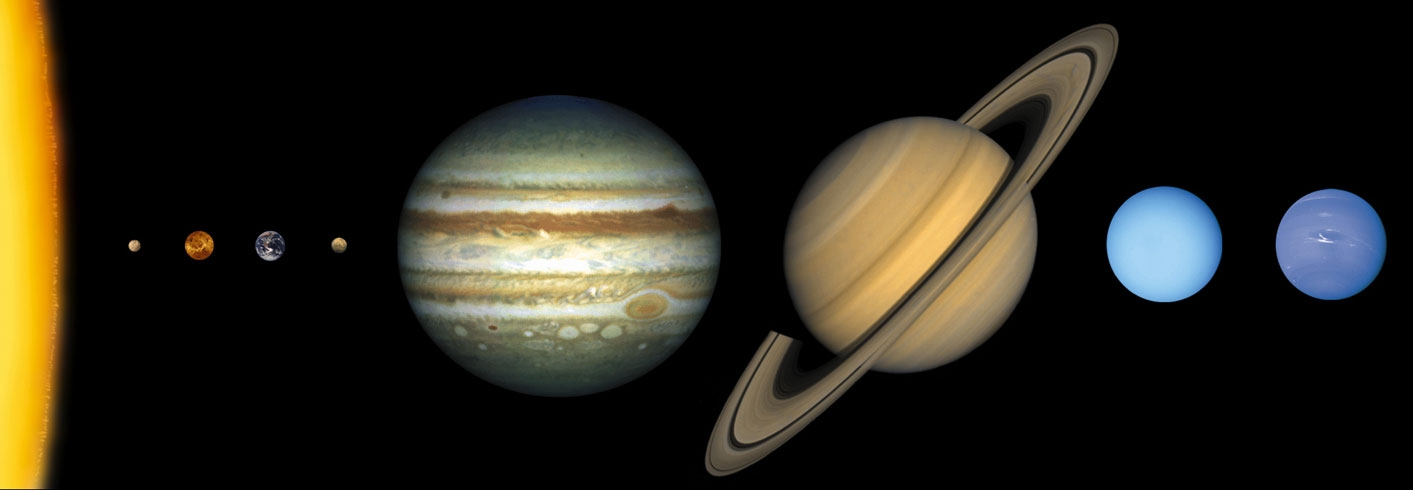
\includegraphics[width=0.9\textwidth{},keepaspectratio]{sun.jpg}
  \caption[fig:sun]{最左侧是太阳,向右依序为水星、金星、地球、火星、
    木星、土星、天王星与海王星}
    \end{figure}

天文学家在太阳系内以天文单位(AU)来测量距离。1AU是地球到太阳的平均距离,
大约是\num{149598000}公里(\num{93000000}英里)。冥王星与太阳的距离大约
是39AU,木星则约是5.2AU。最常用在测量恒星距离的长度单位是光年,1光年大约
相当于\num{63240}天文单位\footnote{维基百科:太阳系}。

图~\ref{fig:sun}展示了太阳系的各行星的位置。

\begin{table}[htbp]
  \caption[tab:xingxing]{行星数据表}
  \centering
  \vspace{0.2cm}
  \zhongwu
  \begin{tabular}{cccc}
    \toprule
    Planet  & Size(Earth=1) & Weight(Earth=1) & Radius  \\
    \midrule
    Mercury & 0.056         & 0.055           & 0.3871  \\
    Venus   & 0.857         & 0.815           & 0.7233  \\
    Earth   & 1.00          & 1.000           & 1.0000  \\
    Mars    & 0.151         & 0.107           & 1.5237  \\
    Jupiter & 1321          & 317.832         & 5.2026  \\
    Saturn  & 755           & 95.16           & 9.5549  \\
    Uranus  & 63            & 14.54           & 19.2184 \\
    Neptune & 58            & 17.15           & 30.1104 \\
    \bottomrule
  \end{tabular}
\end{table}

表~\ref{tab:xingxing}就是最简单的三线表。源代码如下:
\begin{lstlisting}
  \begin{table}[htbp]
    \caption[tab:xingxing]{行星数据表}
        \centering
    \vspace{0.2cm}
    \zhongwu
    \begin{tabular}{cccc}
      \toprule
      Planet  & Size(Earth=1) & Weight(Earth=1) & Radius  \\
      \midrule
      Mercury & 0.056         & 0.055           & 0.3871  \\
      Venus   & 0.857         & 0.815           & 0.7233  \\
      Earth   & 1.00          & 1.000           & 1.0000  \\
      Mars    & 0.151         & 0.107           & 1.5237  \\
      Jupiter & 1321          & 317.832         & 5.2026  \\
      Saturn  & 755           & 95.16           & 9.5549  \\
      Uranus  & 63            & 14.54           & 19.2184 \\
      Neptune & 58            & 17.15           & 30.1104 \\
      \bottomrule
    \end{tabular}
  \end{table}
\end{lstlisting}


表格和插图通常需要占据大块空间,所以在文字处理软件中用户经常需要调整它们的
位置。\texttt{table}环境可以自动完成这样的任务;这种自动调整位置的环境称作
浮动环境 (float),下一节里还会介绍插图浮动环境\footnote{包太雷:\LaTeX{}
  NOTES———雷太赫排版系统简介}。

\texttt{htbp} 选项用来指定表格的理想位置,这几个字母分别代表 here, top,
bottom,float page,也就是就这里、页顶、页尾、浮动页 (专门放浮动环境的单独
页面)。我们可以使用这几个字母的任意组合,四个字母都写上表示放哪里都无所
谓;一般不推荐单独使用h,因为\LaTeX{}自以为它的排版算法是最完美的,不愿意
被束缚手脚。

\texttt{\textbackslash{centering}} 用来使表格居
中;\texttt{\textbackslash{caption}} 命令设置表格标题,\LaTeX{}会自动给
浮动环境的标题加上编号。

它的官方使用说明为:
\begin{lstlisting}
  \caption[label]{ 中文标题 }
  \end{lstlisting}
可选参数~\texttt{\footnotesize label}~用来作为交叉引用链接。例如
表~\ref{tab:xingxing}中的\texttt{lable}为\texttt{tab:xingxing}。这里的标
签一般为英文。中文短标题一般没什么用,可以随意填。最简单就是“表”。

在表格环境中,标题必须位于表格的上方。而在图片环境中,标题的位置必须位于
图片的下方。

\texttt{tabular} 环境提供了最简单的表格功能。它用 \texttt{\&} 来分列,
用 \texttt{\textbackslash{\textbackslash{}}} 来换行;每列可以采用居中、居
左、居右等横向对齐方式,分别用 \texttt{l、c、r} 来表示。

三线表的三条横线就分别
用 \texttt{\textbackslash{toprule}}、\texttt{\textbackslash{midrule}}、
\texttt{\textbackslash{bottomrule}} 等命令表示。

\texttt{\textbackslash{vspace}\{0.2cm\}}是用来控制表格标题与表格正文的
垂直间距的,请在插入表格时务必添加。\texttt{\textbackslash{zhongwu}}是
用来调整表格内容的行距的。


\BiSubsection{表格的列按小数点对齐}{XXX}

以表~\ref{tab:xingxing}为例,想把其中的第三列按小数点对齐\footnote{参见宏
  包siunitx}。先看一下效果:

在表~\ref{tab:xiaoshu}中,我们调整了原来四列数的对齐方式。原来
是\texttt{cccc},现在是\texttt{lcSr}。第一列左对齐,第二列不变,还是居中
对齐,第四列右对齐。值得注意的是第三列,这里新引入了一个参数\texttt{S},
含义就是这一列的数字按照小数点对齐。一定是大写的S。另外,第三列的列
头Weight(Earth=1)两边也加上了大括号,因为这不是数字。在使用参
数\texttt{S}的时候,不是数字的行需要用大括号括起来,不然会造成编译错误。

\begin{table}[htbp]
  \caption[tab:xiaoshu]{行星数据表}
  \centering
  \vspace{0.2cm}
  \zhongwu
  \begin{tabular}{lcSr}
    \toprule
    Planet  & Size(Earth=1) & {Weight(Earth=1)} & Radius  \\
    \midrule
    Mercury & 0.056         & 0.055           & 0.3871  \\
    Venus   & 0.857         & 0.815           & 0.7233  \\
    Earth   & 1.00          & 1.000           & 1.0000  \\
    Mars    & 0.151         & 0.107           & 1.5237  \\
    Jupiter & 1321          & 317.832         & 5.2026  \\
    Saturn  & 755           & 95.16           & 9.5549  \\
    Uranus  & 63            & 14.54           & 19.2184 \\
    Neptune & 58            & 17.15           & 30.1104 \\
    \bottomrule
  \end{tabular}
\end{table}

\begin{lstlisting}
  \begin{table}[htbp]
    \caption[tab:xiaoshu]{ 行星数据表 }
    \centering
    \vspace{0.2cm}
    \zhongwu
    \begin{tabular}{lcSr}
      \toprule
      Planet  & Size(Earth=1) & {Weight(Earth=1)} & Radius  \\
      \midrule
      Mercury & 0.056         & 0.055           & 0.3871  \\
      Venus   & 0.857         & 0.815           & 0.7233  \\
      Earth   & 1.00          & 1.000           & 1.0000  \\
      Mars    & 0.151         & 0.107           & 1.5237  \\
      Jupiter & 1321          & 317.832         & 5.2026  \\
      Saturn  & 755           & 95.16           & 9.5549  \\
      Uranus  & 63            & 14.54           & 19.2184 \\
      Neptune & 58            & 17.15           & 30.1104 \\
      \bottomrule
    \end{tabular}
  \end{table}
\end{lstlisting}

\BiSubsection{多列三线表}{XXXXXX}

在三线表中,有些列的列头会横跨好几列的数据。一般使
用\texttt{multicolumn}命令。它的用法是:
\begin{lstlisting}
  \multicolumn{ 列数}{ 对齐方式 }{ 表格内容 }
\end{lstlisting}

“列数”是指这一列横跨的列数,在表~\ref{tab:linux}是2列,就填“2”;“对
齐方式”从\texttt{lcr}三者中选其一即可,在表~\ref{tab:linux}中是c。“表格
内容”填入自己的内容。一般还会在这一列的下面画一小横线,已示辨识。使
用\texttt{cmidrule}命令。在表~\ref{tab:linux}中,由于横跨的是第2列和第3列,
因此\texttt{cmidrule}的参数是2-3。

\begin{table}[htbp]
  \caption[tab:linux]{ 不同操作系统下的\LaTeX{} }
  \centering
  \vspace{0.2cm}
  \zhongwu
  \begin{tabular}{ccc}
    \toprule
    Test    & \multicolumn{2}{c}{Common Tools} \\
    \cmidrule{2-3}
    OS         & Distribution & Editor            \\
    \midrule
    Windows    & MikTeX       & TexMakerX         \\
    Mac OS     & MacTeX       & TeXShop           \\
    Linux/Unix & TeX Live     & TeXworks          \\
    \bottomrule
  \end{tabular}
\end{table}


\begin{lstlisting}
  \begin{table}[htbp]
    \caption[tab:linux]{ 不同操作系统下的\LaTeX{}}
    \centering
    \vspace{0.2cm}
    \zhongwu
    \begin{tabular}{ccc}
      \toprule
      Test    & \multicolumn{2}{c}{Common Tools} \\
      \cmidrule{2-3}
      OS         & Distribution & Editor            \\
      \midrule
      Windows    & MikTeX       & TexMakerX         \\
      Mac OS     & MacTeX       & TeXShop           \\
      Linux/Unix & TeX Live     & TeXworks          \\
      \bottomrule
    \end{tabular}
  \end{table}
\end{lstlisting}

\BiSubsection{多行三线表}{XXXXXXXX}

既然有多列三线表,多行三线表也是用类似的方法解决。我们把表~\ref{tab:linux} 来改造一下,相对应的,一般使用\texttt{multirow}命令。它的用法
是:
\begin{lstlisting}
  \multirow{ 行数 }*{ 表格内容 }
\end{lstlisting}

“行数”是指竖向跨的行数,在表~\ref{tab:unix}中是2行,中间有个星号,表示自然宽度。

\begin{table}[htbp]
  \caption[tab:unix]{ 不同操作系统下的\LaTeX{} }
  \centering
  \vspace{0.2cm}
  \zhongwu
  \begin{tabular}{ccc}
    \toprule
    \multirow{2}*{OS} & \multicolumn{2}{c}{Common Tools} \\
    \cmidrule{2-3}
    & Distribution & Editor            \\
    \midrule
    Windows          & MikTeX       & TexMakerX         \\
    Mac OS           & MacTeX       & TeXShop           \\
    Linux/Unix       & TeX Live     & TeXworks          \\
    \bottomrule
  \end{tabular}
\end{table}


\begin{lstlisting}
  \begin{table}[htbp]
    \caption[tab:unix]{ 不同操作系统下的\LaTeX{} }
    \centering
    \vspace{0.2cm}
    \zhongwu
    \begin{tabular}{ccc}
      \toprule
      \multirow{2}*{OS} & \multicolumn{2}{c}{Common Tools} \\
      \cmidrule{2-3}
      & Distribution & Editor            \\
      \midrule
      Windows          & MikTeX       & TexMakerX         \\
      Mac OS           & MacTeX       & TeXShop           \\
      Linux/Unix       & TeX Live     & TeXworks          \\
      \bottomrule
    \end{tabular}
  \end{table}
\end{lstlisting}

\BiSubsection{宽度控制}{SDADASDAS}

有时候表格中的某行太长了,需要折行。可以使用\texttt{tabularx} 宏包的同名
环境,其语法如下:

\begin{lstlisting}
  \begin{tabularx}{ 表格总宽度 }{ 对齐方式 }
    ...
  \end{tabularx}
\end{lstlisting}

“表格总宽度”最好用\texttt{textwidth}乘以某个系数表示。例
如\texttt{0.8\textbackslash{textwidth}}表示表格宽度是版芯宽度的0.8倍。这
样出来的效果比较好看。对齐方式除了原有的\texttt{l,c,r}之外,多了一
个\texttt{X},表示某列可以折行。

\begin{table}[htbp]
  \centering
  \caption[tab:wall]{ 墙上的44句话 }
  \vspace{0.2cm}
  \zhongwu
  \begin{tabularx}{0.8\textwidth{}}{lX}
    \toprule
    People & Says \\
    \midrule
    Elias Canetti & If you were alone, you would cut yourself in two, so
    that one part would shape the other.\\
    Franz Kafka & In the struggle between yourself and the world,
    second the world.\\
    \bottomrule
  \end{tabularx}
\end{table}

\begin{lstlisting}
  \begin{table}[htbp]
    \centering
    \caption[tab:figure]{ 墙上的44句话 }
    \vspace{0.2cm}
    \zhongwu
    \begin{tabularx}{0.8\textwidth{}}{lX}
      \toprule
      People & Says \\
      \midrule Elias Canetti & If you were alone, you would cut yourself
      in two, so  that one part would shape the other.\\
      Franz Kafka & In the struggle between yourself and the world,
      second the world.\\
      \bottomrule
    \end{tabularx}
  \end{table}
\end{lstlisting}



\BiSubsection{斜线表头}{DASDFSAFASF}

还是有些童鞋的表示三线表不实用啊,非要回归到原来的斜线表头去。我们可以使
用宏包\texttt{diagbox}提供的命令轻松完成。不过呢,出来的表格很ugly罢了。

\texttt{diagbox}是宏包提供的主要命令。它可以带有两个必选参数,表示要生成斜
线表头的两部分内容。默认斜线是从西北到东南方向的。

需要注意的是,使用斜线表格后就不能使用三线表的三条横线,不然请看
表~\ref{tab:diagbox}的下场。正确的做法是使用最原始的\texttt{hline},见
表~\ref{tab:xiexian}。

\begin{table}[htbp]
  \caption[tab:diagbox]{斜线表头}
  \centering
  \vspace{0.2cm}
  \zhongwu
  \begin{tabular}{|l|ccc|}
    \toprule
    \diagbox{Times}{Day} & Mon  & Tue  & Wed  \\
    \midrule
    Morning              & used & used &      \\
    Afternoon            &      & used & used \\
    \bottomrule
  \end{tabular}
\end{table}

\begin{lstlisting}
  \begin{table}[htbp]
    \caption[tab:diagbox]{ 斜线表头 }
    \centering
    \vspace{0.2cm}
    \zhongwu
    \begin{tabular}{|l|ccc|}
      \toprule
      \diagbox{Times}{Day} & Mon  & Tue  & Wed  \\
      \midrule
      Morning              & used & used &      \\
      Afternoon            &      & used & used \\
      \bottomrule
    \end{tabular}
  \end{table}
\end{lstlisting}

\begin{table}[htbp]
  \caption[tab:xiexian]{斜线表头}
  \centering
  \vspace{0.2cm}
  \zhongwu
  \begin{tabular}{|l|ccc|}
    \hline
    \diagbox{Times}{Day} & Mon  & Tue  & Wed  \\
    \hline
    Morning              & used & used &      \\
    Afternoon            &      & used & used \\
    \hline
  \end{tabular}
\end{table}

\begin{lstlisting}
  \begin{table}[htbp]
    \caption[tab:xiexian]{ 斜线表头 }
    \centering
    \vspace{0.2cm}
    \zhongwu
    \begin{tabular}{|l|ccc|}
      \hline
      \diagbox{Times}{Day} & Mon  & Tue  & Wed  \\
      \hline
      Morning              & used & used &      \\
      Afternoon            &      & used & used \\
      \hline
    \end{tabular}
  \end{table}
\end{lstlisting}


\BiSection{图}{Figures}
\label{chap02:figure}

我来北京十一年,上学,上班,也积累了不少同学同事,但我一次他们的婚礼都没
有参加过。刚毕业的时候这种邀请很多,好象是种翻天覆地日新月异的见证,不怕
那些同学们伤心,我也知道人家是真心邀请的,但我真觉得我没跟他们谁好到真有
必要参加那些婚礼,所以我就不去。这次黄总的婚礼通知的突然,但我却很想去见
证一下,我的罪恶太多,正好也让天主顺便宽恕宽恕我,沾沾喜气\footnote{蚌病
  生珠:阳光下的婚礼}。

我挺佩服黄总他们俩的,他们就真的仅仅在婚礼当天才拍所谓的“婚纱照”。我觉
得这样挺好。身为摄影部的美女,周围全是靠摄影吃饭的人,的确没必要出去花冤
枉钱就为了拍几张照片。

\begin{figure}[htbp]
  \centering
  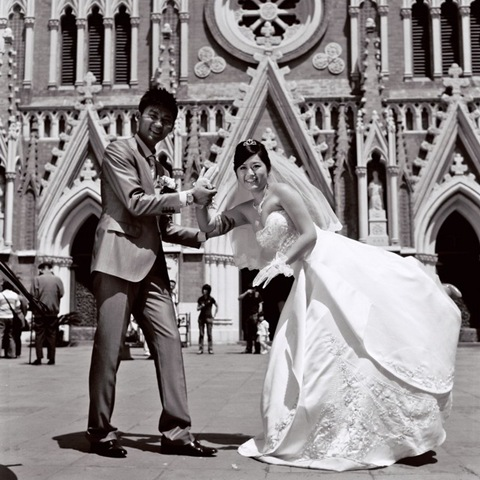
\includegraphics[scale=0.6]{wedding.jpg}
  \caption[fig:wedding]{婚礼}
\end{figure}

\begin{lstlisting}
  \begin{figure}[htbp]
    \centering
    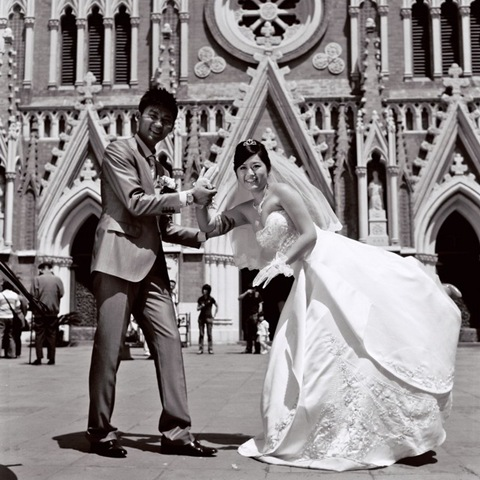
\includegraphics[scale=0.6]{wedding.jpg}
    \caption[fig:wedding]{ 婚礼 }
  \end{figure}
\end{lstlisting}

论文使用的图片都放在figure文件夹中,插图浮动环境是\texttt{figure},基本命
令是\texttt{includegraphics},而在图片环境中,标题的位置必须位于图片的下
方。

\texttt{includegraphics}的基本参数见表~\ref{tab:figure}。

\begin{table}[htbp]
  \centering
  \caption[tab:figure]{插图命令参数}
  \vspace{0.2cm}
  \zhongwu
  \begin{tabularx}{0.8\textwidth{}}{lX}
    \toprule
    参数             & 说明 \\
    \midrule
    width=x,height=y & 宽度和高度,绝对尺寸,可用任意长度单位。                           \\
    scale=s          & 缩放比。绝对尺寸和缩放比用一种即可,同时使用两者,绝对尺寸起作用。 \\
    keepaspectratio & 保持图形比例。宽度和高度通常设置一个即可,否则图形比
    例会失调,除非再加上此选 项,
    这样图形宽度和高度都不超过指定参数。                                                \\
    angle=a          & 逆时针旋转角度,单位是度。                                        \\
    \bottomrule
  \end{tabularx}
\end{table}

对于图~\ref{fig:wedding},只使用了\texttt{scale}这一个参数,缩放因子是0.6。
当然,也可以直接指定图形的宽度和高度。图~\ref{fig:sun}的源代码如下:

\begin{lstlisting}
  \begin{figure}[htbp]
    \centering
    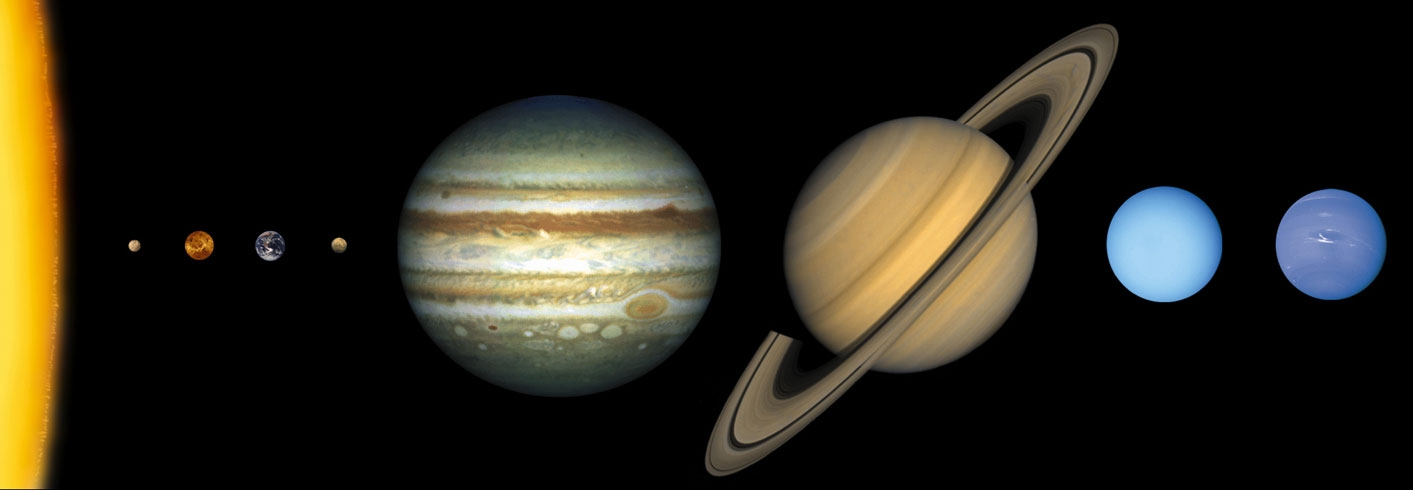
\includegraphics[width=\textwidth{},keepaspectratio]{sun.jpg}
    \caption[fig:sun]{ 最左侧是太阳,向右依序为水星、金
      星 }
  \end{figure}
\end{lstlisting}

可以看到,图~\ref{fig:sun}的宽度指定为版芯的宽度,然后使用了保持宽高比这
个选项。


\BiSubsection{双图并列}{Two Figures}

温文敦厚的新郎,美丽可爱的新娘。

Alan和Cher这一对从校园时代就相偎相依一直到步入婚礼的殿堂。

我一直觉得,这样的情侣是最最难得的,两个人之间最珍贵的东西得以一直保存、
延续,直至在未来某个时候升华成为生命中不可名状的一种记忆和体验。这个世界
上有太多因为坚持或者不坚持,执着或者不执着导致的有始无终。能够沿路陪伴,
最终成为眷属,也算是不大不小的奇迹。

两个人的婚礼誓词很肉麻,很感人,写在小纸片上,认真的读出来,直到读到对方
流下感动的泪水,直到在场的嘉宾都用掌声回应这份真情\footnote{蚌病生珠:罗
  兰湖畔}。

\begin{figure}[htbp]
  \centering
  \begin{minipage}{0.4\textwidth}
    \centering
    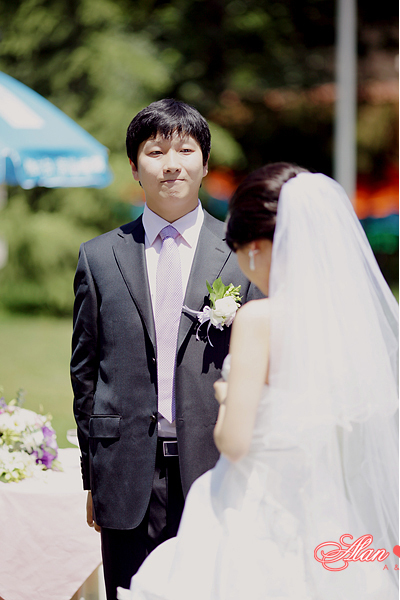
\includegraphics[keepaspectratio]{lang.jpg}
    \caption[fig:lang]{新郎}
  \end{minipage}
  \begin{minipage}{0.4\textwidth}
    \centering
    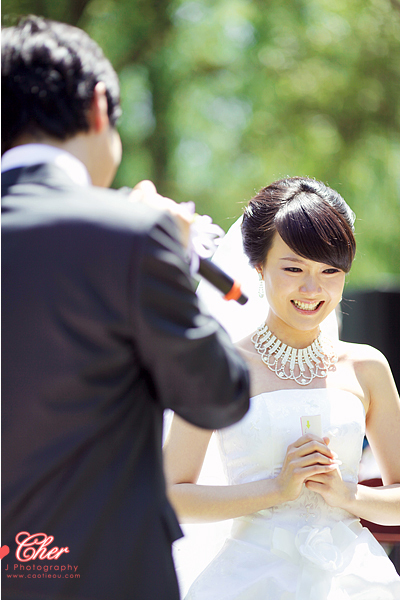
\includegraphics[keepaspectratio]{liang.jpg}
    \caption[fig:niang]{新娘}
  \end{minipage}
\end{figure}

\begin{lstlisting}
  \begin{figure}[htbp]
    \centering
    \begin{minipage}{0.4\textwidth}
      \centering
      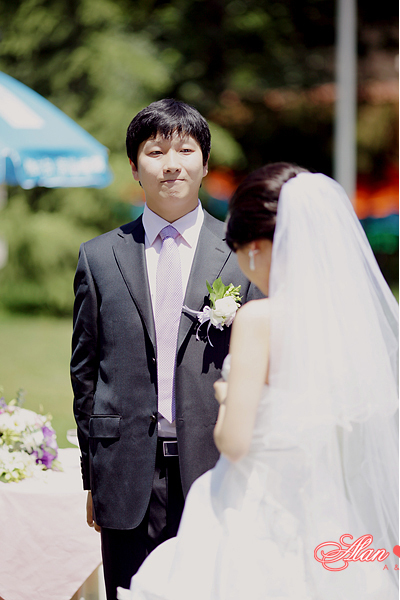
\includegraphics[keepaspectratio]{lang.jpg}
      \caption[fig:lang]{ 新郎 }
    \end{minipage}
    \begin{minipage}{0.4\textwidth}
      \centering
      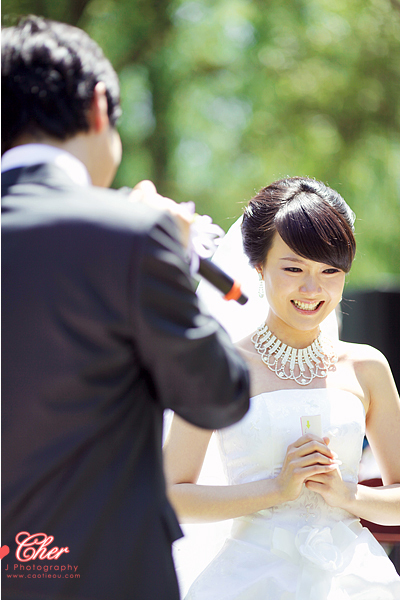
\includegraphics[keepaspectratio]{liang.jpg}
      \caption[fig:niang]{ 新娘 }
    \end{minipage}
  \end{figure}
\end{lstlisting}


如果想要两幅并排的插图各有自己的标题,可以在 figure 环境中使用两
个 \texttt{minipage} 环境,每个里面插入一幅图 (见图~\ref{fig:lang}和
图~\ref{fig:niang}) 。不用 \texttt{minipage} 的话,因为插图标题的缺省宽度是
整个行宽;两幅插图就会上下排列。

这里指定了每个\texttt{minipage}的宽度为0.4倍的版芯宽度。当然,也可以自
己指定,只是两个宽度加起来不超过版芯宽度就可以了。


\BiSubsection{两子图并列}{Two subfigures}

有你在,开水瓶里永远都有水喝;冰箱里永远有一袋应急的速冻饺子;阳台的晾衣
架上我昨天换下的衣服已经有了今天太阳的味道;小猫也不用害怕得病和不舒服,
它们有最负责任的家庭医生;还有别人根本见都没见过的那些点心和饼干;还有,
你是我见过的少有的照片和本人都好看的女孩\footnote{蚌病生珠:Two-year
  anniversary}。


\begin{figure}[htbp]
  \centering
  \subfigure[超人A]{
    \label{fig:1a}
    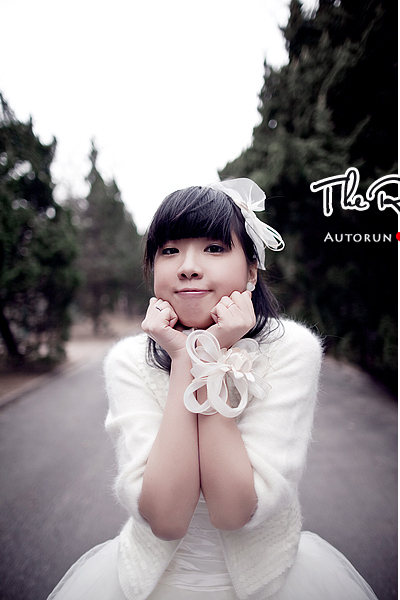
\includegraphics[keepaspectratio]{chao.jpg}
  }
  \hspace{20pt}
  \subfigure[超人A]{
    \label{fig:1b}
    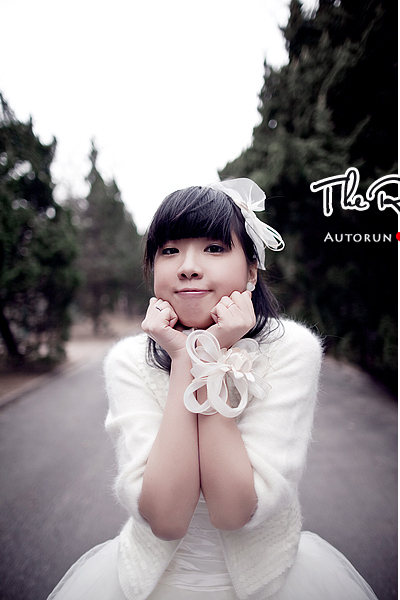
\includegraphics[keepaspectratio]{chao.jpg}
  }
  \caption[fig:judy]{小超人老师}
\end{figure}

\begin{lstlisting}
  \begin{figure}[htbp]
    \centering
    \subfigure[超人A]{
      \label{fig:1a}
      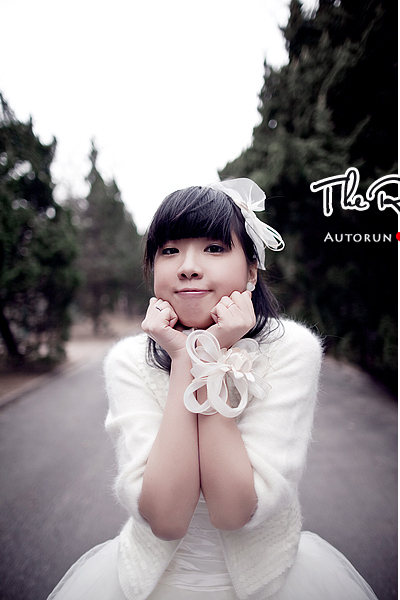
\includegraphics[keepaspectratio]{chao.jpg}
    }
    \hspace{20pt}
    \subfigure[超人A]{
      \label{fig:1b}
      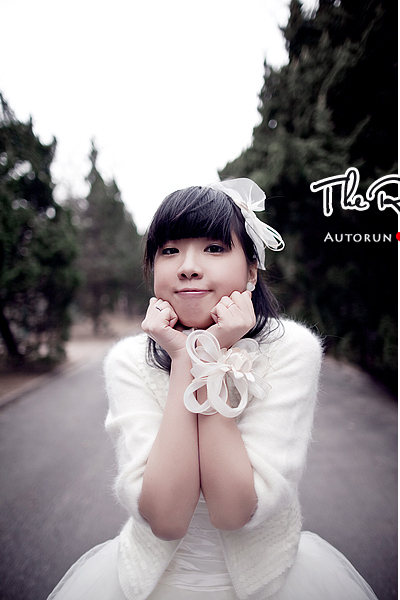
\includegraphics[keepaspectratio]{chao.jpg}
    }
    \caption[fig:judy]{小超人老师}
  \end{figure}
\end{lstlisting}

如果想要两幅并排的图片共享一个标题,并且各有自己的子标题,可以使
用\texttt{subcaption}宏包。如图~\ref{fig:judy},子图的标题用命令
\texttt{subcaption}即可。

\BiSection{数学}{Mathematics}

\BiSubsection{math}{math}

$\mathbf{A},\mathcal{A},\mathfrak{A},\mathbb{A}$

\begin{lstlisting}
  $\mathbf{A},\mathcal{A},\mathfrak{A},\mathbb{A}$
\end{lstlisting}

\BiSubsection{傅立叶变换}{Fourier transform }

在现代数学中有一个很容易被外行误解的词汇:信号 (signal)。当数学家们说起
「一个信号」的时候,他们脑海中想到的并不是交通指示灯所发出的闪烁光芒或者
手机屏幕顶部的天线图案,而是一段可以具体数字化的信息,可以是声音,可以是
图像,也可是遥感测量数据。简单地说,它是一个函数,定义在通常的一维或者多
维空间之上。譬如一段声音就是一个定义在一维空间上的函数,自变量是时间,因
变量是声音的强度,一幅图像是定义在二维空间上的函数,自变量是横轴和纵轴坐
标,因变量是图像像素的色彩和明暗,如此等等\footnote{木遥:不确定性原理的
  前世今生 · 数学篇(一)}。

在数学上,关于一个信号最基本的问题在于如何将它表示和描述出来。按照上面所
说的办法,把一个信号理解成一个定义在时间或空间上的函数是一种自然而然的表
示方式,但是它对理解这一信号的内容来说常常不够。例如一段声音,如果单纯按
照定义在时间上的函数来表示,它画出来是这个样子的:

\begin{figure}[htbp]
  \centering
  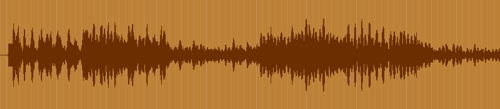
\includegraphics[width=0.8\textwidth{},keepaspectratio]{VisualAudio.png}
  \caption[fig:boxingtu]{波形图}
\end{figure}

图~\ref{fig:boxingtu}通常被称为波形图。毫无疑问,它包含了关于这段声音的全
部信息。但是同样毫无疑问的是,这些信息几乎没法从上面这个「函数」中直接看
出来,事实上,它只不过是巴赫的小提琴无伴奏 Partita No.3 的序曲开头几个小
节。图~\ref{fig:bahe} 是巴赫的手稿,从某种意义上说来,它也构成了对上面那
段声音的一个「描述」:

\begin{figure}[htbp]
  \centering
  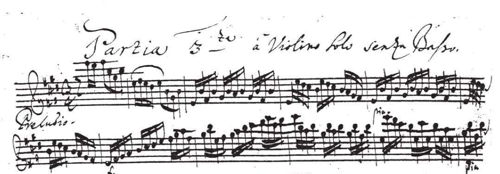
\includegraphics[width=0.8\textwidth{},keepaspectratio]{Partita3.png}
  \caption[fig:bahe]{巴赫手稿}
\end{figure}

这两种描述之间的关系是怎样的呢?第一种描述刻划的是具体的信号数值,第二种
描述刻划的是声音的高低(即声音震动的频率)。人们直到十九世纪才渐渐意识到,
在这两种描述之间,事实上存在着一种对偶的关系,而这一点并不显然。

1807 年,法国数学家傅立叶 (J. Fourier) 提出了一个崭新的观念:任何一个函数
都可以表达为一系列不同频率的简谐振动(即简单的三角函数)的叠加。

用今天的语言来描述,傅立叶的发现实际上是在说:任何一个信号都可以用两种方
式来表达,一种就是通常意义上的表达,自变量是时间或者空间的坐标,因变量是
信号在该处的强度,另一种则是把一个信号「展开」成不同频率的简单三角函数
(简谐振动)的叠加,于是这就相当于把它看作是定义在所有频率所组成的空间
(称为频域空间)上的另一个函数,自变量是不同的频率,因变量是该频率所对应
的简谐振动的幅度。


这两个函数一个定义在时域(或空域)上,一个定义在频域上,看起来的样子通常
截然不同,但是它们是在以完全不同的方式殊途同归地描述着同一个信号。它们就
象是两种不同的语言,乍一听完全不相干,但是其实可以精确地互相翻译。在数学
上,这种翻译的过程被称为「傅立叶变换」。

傅立叶变换是一个数学上极为精美的对象:
\begin{enumerate}
\item 它是完全可逆的,任何能量有限的时域或空域信号都存在唯一的频域表达,
  反之亦然 。
\item 它完全不损伤信号的内在结构:任何两个信号之间有多少相关程度(即内
  积),它们的频域表达之间也一定有同样多的相关程度。
\item 它不改变信号之间的关联性:一组信号收敛到一个特定的极限,它们的频域
  表达也一定收敛到那个极限函数的频域表达。
\end{enumerate}

在傅立叶变换的所有这些数学性质中,最不寻常的是这样一种特性:一个在时域或
空域上看起来很复杂的信号(譬如一段声音或者一幅图像)通常在频域上的表达会
很简单。这里「简单」的意思是说作为频域上的函数,它只集中在很小一块区域内,
而很大一部分数值都接近于零。

一个在空域中看起来占满全空间的信号,从频域中看起来很可能只不过占用了极小
一块区域,而大部分频率是被浪费了的。这就导出了一个极为有用的结论:一个看
起来信息量很大的信号,其实可以只用少得多的数据来加以描述。只要对它先做傅
立叶变换,然后只记录那些不接近零的频域信息就可以了,这样数据量就可以大大
减少。

基本上,这正是今天大多数数据压缩方法的基础思想。在互联网时代,大量的多媒
体信息需要在尽量节省带宽和时间的前提下被传输,所以数据压缩从来都是最核心
的问题之一。而今天几乎所有流行的数据压缩格式,无论是声音的 mp3 格式还是图
像的 jpg 格式,都是利用傅立叶变换才得以发明的。从这个意义上说来,几乎全部
现代信息社会都建立在傅立叶的理论的基础之上。



\BiSection{参考文献}{References}


硕士论文写了3周。90多页英文,昏天黑地没日没夜写到想吐。好在有几个欧洲博士
后帮忙改语法错。改的他们也很想哭。后来已经功成名就论文无数ACM
Fellow英国Fellow of Royal Society的老板来给我们讲,写论文最重要的是
写Introduction。写Introduction就和写童话一样\footnote{珵cici:硕士论文你有
  哪些经验与收获?耗時多久?}。

\begin{enumerate}[1.]
\item 有一条巨龙抓走了公主 (介绍你的问题为什么值得研究)
\item 巨龙是多么多么多么难打(强调你的研究的重要性)
\item 王子提着一把金光闪闪的剑而不是破斧子烂长矛登场(你的方法好在哪里,别人sui在哪里)
\item 王子是如何打败巨龙(你的方法简介)
\item 从此王子和公主幸福的生活在一起。(解决了问题)
\end{enumerate}

老板说写论文就是写童话嘛。其余的也不过就是把这些东西细节讲一讲。做研究很
简单的。听完我就不想再做研究了。合着我写到吐血掉头发的时候大牛都把写论文
当给小盆友写童话。


我们的一切知识都是从经验开始\cite{李秋零1999},这是没有任何怀疑的\cite{邓晓芒2005}\cite{邓晓芒2000};
因为,如果不是对象激动我们的感官,一则由它们自己引起表象,一则使我们的知性活动运作起来,对这些表象加
以比较,把它们粘结或分开,\cite{欧进萍1999,欧进萍1991}这样把感性印象的原始素材加工成称之为经验的对象
知识,那么知识能力又该由什么来唤起活动呢?\cite{braun2007,kelton2002,strawderman2001,李秋零1999}所以
按照时间,我们没有任何知识是先行于经验的,一切知识都是从经验开始的。

学位论文参考第一个的格式。\cite{温雅静2014}


只要是中文文献,图书,期刊,会议,专利等等需要为每个条目增加一个域:
\begin{lstlisting}
  language={c},
\end{lstlisting}

对于参考文献[1],原先的bib文件是这样的:
\begin{lstlisting}
  @article{ 李秋零1999 ,
    title={ 康德何以步安瑟尔谟的后尘? },
    author={ 李秋零 },
    journal={ 中国人民大学学报 },
    volume={2},
    year={1999}
  }
\end{lstlisting}


但是由于是中文文献,需要增加一个语言域,就变成下列样式:
\begin{lstlisting}
  @article{ 李秋零1999,
    title={ 康德何以步安瑟尔谟的后尘? },
    author={ 李秋零 },
    language={c},
    journal={ 中国人民大学学报 },
    volume={2},
    year={1999}
  }
\end{lstlisting}
% !TEX TS-program = XeLaTeX
% !TEX encoding = UTF-8 Unicode

\BiChapter{注意事项}{Notes}
%\label{chap03}
\BiSection{引~~言}{Introduction}
请直接双面打印PDF文件,空白页已经按要求留出。打印时,缩放页面的选项设
为“无”,否则页面会缩小。

参考文献的bib文件的条目的名称是不允许出现空格的。

% 结论
% !TEX TS-program = XeLaTeX
% !TEX encoding = UTF-8 Unicode

\BiChapter{结论与展望}{The Summarize and Prospect}


该部分主要包括两部分:“结论”和“展望”。结论是理论分析和实验结果的逻辑发展,是整篇论文的归宿。结论是在理论分析、试验结果的基础上,经过分析、推理、判断、归纳的过程而形成的总观点。结论必须完整、准确、鲜明、并突出与前人不同的新见解。总结部分还应说明论文中的创新点内容。创新点应该以分条列举的形式进行提出。展望是对该研究课题存在的不足和有待改进的说明,是对未来研究的一种期待。该部分的字数应不少于半页。

书写格式说明:
标题“结论与展望”选用模板中的样式所定义的“结论与展望”,或者手动设置成字体:黑体,居中,字号:小三,1.5倍行距,段后1行,段前为0行。
结论正文选用模板中的样式所定义的“正文”,每段落首行缩进2字;或者手动设置成每段落首行缩进2字,字体:宋体,字号:小四,行距:多倍行距 1.25,间距:前段、后段均为0行。

\cleardoublepage
\backmatter

% 参考文献
\addcontentsline{toc}{chapter}{参考文献}
\addcontentsline{toe}{chapter}{References} % 参考文献加入到英文目录 by zzupc
\defaultfont
\wuhao
\bibliographystyle{zjugbno}
\bibliography{body/reference}
\cleardoublepage
% 附录
\defaultfont
\begin{appendix}
  % !TEX TS-program = XeLaTeX
% !TEX encoding = UTF-8 Unicode

\chapter*{\hfill 附录~A 附录\hfill} %手动加入双语目录
\addcontentsline{toc}{chapter}{附录~A 附录}
\addcontentsline{toe}{chapter}{The Appendix content A  Appendix content name}
\renewcommand{\thetable}{A.\arabic{table}}
\renewcommand{\thefigure}{A.\arabic{figure}}
\renewcommand{\theequation}{A\arabic{equation}}

以下内容可放在附录之内:

\begin{asparaenum}
\item 正文内过于冗长的公式推导;
\item 方便他人阅读所需的辅助性数学工具或表格;
\item 重复性数据和图表;
\item 论文使用的主要符号的意义和单位;
\item 程序说明和程序全文。
\end{asparaenum}

这部分内容可省略。
\end{appendix}
\cleardoublepage

\defaultfont
% 发表的文章列表
%% !TEX TS-program = XeLaTeX
% !TEX encoding = UTF-8 Unicode

%%%%%%%%%%%%%%%%%%%%%%%%%%%%%%%%%%%%%%%%%%%%%%%%%%%%%%%%%%%%%%%%%%%%%
%
%	大连理工大学博士论文 XeLaTeX 模版 —— 发表论文文件 publications.tex
% 版本:0.8
% 最后更新:2012.04.04
% 修改者:Yuri (E-mail: yuri_1985@163.com)
% 修订者:whufanwei(E-mail: dutfanwei@qq.com)
% 编译环境1:Ubuntu 12.04 + TeXLive 2011 + Emacs
% 编译环境2:Windows 7 + CTeX v2.9.2.164 + WinEdit
%
%%%%%%%%%%%%%%%%%%%%%%%%%%%%%%%%%%%%%%%%%%%%%%%%%%%%%%%%%%%%%%%%%%%%%

\chapter*{\hfill 攻读博士学位期间科研项目及科研成果 \hfill}
\addcontentsline{toc}{chapter}{攻读博士学位期间科研项目及科研成果}
\addcontentsline{toe}{chapter}{Achievements}
%仅列出博士生攻读博士学位期间发表与学位论文有关的学术论文,
%并注明属于学位论文内容的部分(章节),
%所有作者及其顺序、所发表的刊物名称(包括主办单位、是否被SCI、EI检索期刊)、时间、期号与页码。
%其他时间或与学位论文内容(章节)无关的论文不得列出。示例如下:
首先列出博士生攻读博士学位期间发表与学位论文有关的学术论文,并注明属于学位论文内容的部分(章节),所有作者及其顺序、所发表的刊物名称(包括主办单位、是否被SCI、EI检索期刊)、时间、期号与页码。其他时间或与学位论文内容(章节)无关的论文不得列出。特别声明:对于已经投稿但是没有确认被接受的论文不得写入论文中,列出的论文只能是已经确定发表或者已经确认接收的论文。

其次列出在攻读博士学位期间参与的科研项目(如国家自然科学基金或国家“863”计划等),以及在这期间取得的科研成果(申请的发明专利、在国家级赛事中取得的优异成绩等)。

书写格式说明:
标题“攻读博士学位期间科研项目及科研成果”选用模板中的样式所定义的“发表学术论文情况”;或者手动设置成字体:黑体,居中,字号:小三,1.5倍行距,段后1行,段前为0行。

“攻读博士学位期间科研项目及科研成果”正文选用模板中的样式所定义的“正文”,每段落首行缩进2字;或者手动设置成每段落首行缩进2字,字体:宋体,字号:小四,行距:多倍行距 1.25,间距:前段、后段均为0行。


%\renewcommand{\labelenumi}{[\arabic{enumi}]}



\section*{\underline{攻读博士学位期间发表的学术论文}}
\begin{publist}
\item L. Wang, S. Kang, H. Shum, G. Xu, Error Analysis of Pure
  Rotation-based Self-Calibration, {\em{IEEE Transactions on Pattern
      Analysis and Machine Intelligence (PAMI)}}, in press
\item ×××,××,×××. 一种基于全景图的三维房间导航方法.
  软件学报, 2002, 13(Suppl.): 31-35
\end{publist}


%\section*{在国际和国内学术刊物上发表的论文}
%\begin{enumerate}[label={[\arabic*]}]
%\item L. Wang, S. Kang, H. Shum, G. Xu, Error Analysis of Pure
%  Rotation-based Self-Calibration, {\em{IEEE Transactions on Pattern
%      Analysis and Machine Intelligence (PAMI)}}, in press
%\item ×××,××,×××. 一种基于全景图的三维房间导航方法.
%  软件学报, 2002, 13(Suppl.): 31-35
%\end{enumerate}
%
%\section*{在国际和国内学术会议上发表的论文}
%\begin{enumerate}[label={[\arabic*]}]
%\item L. Wang, S. Kang, H. Shum, G. Xu, Error Analysis of Pure
%  Rotation-based Self-Calibration, {\em{in Proceedings of the Eighth
%      IEEE International Conference on Computer Vision(ICCV'01)}}, I:
%  464-471, Vancouver, BC, Canada, July, 2001
%\item L. Wang, X. Liu, L. Xia, G. Xu, A. Bruckstein, Image
%  Orientation Detection with Integrated Human Perception Cues,
%  {\em{in Proceedings of IEEE International Conference on Image
%      Processing (ICIP'03)}}, in press
%\end{enumerate}




%\cleardoublepage
% 致谢
% !TEX TS-program = XeLaTeX
% !TEX encoding = UTF-8 Unicode

%%%%%%%%%%%%%%%%%%%%%%%%%%%%%%%%%%%%%%%%%%%%%%%%%%%%%%%%%%%%%%%%%%%%%
%
%	大连理工大学硕士论文 XeLaTeX 模版 —— 致谢文件 acknowledgements.tex
%	版本:0.71
%	最后更新:2010.12.22
%	修改者:Yuri (E-mail: yuri_1985@163.com)
%	编译环境:Ubuntu 10.04 + TeXLive 2010 + TeXworks
%             Windows XP SP3 + CTeXLive 2009 + WinEdt 5.6
%
%%%%%%%%%%%%%%%%%%%%%%%%%%%%%%%%%%%%%%%%%%%%%%%%%%%%%%%%%%%%%%%%%%%%%

\chapter*{\hfill 致  谢 \hfill}
\addcontentsline{toc}{chapter}{致  谢}
\addcontentsline{toe}{chapter}{Acknowledgements}
学位论文中不得书写与论文工作无关的人和事,对导师的致谢要实事求是。

一同工作的同志对本研究所做的贡献应在论文中做明确的说明并表示谢意。

这部分内容不可省略。

在这里,向所有协助测试的同学、朋友表示感谢。
\cleardoublepage
% 作者简介
%% !TEX TS-program = XeLaTeX
% !TEX encoding = UTF-8 Unicode

%%%%%%%%%%%%%%%%%%%%%%%%%%%%%%%%%%%%%%%%%%%%%%%%%%%%%%%%%%%%%%%%%%%%%%
%
%	大连理工大学博士论文 XeLaTeX 模版 —— 作者介绍 about.tex
%	版本:0.71
%	最后更新:2010.12.22
%	修改者:Yuri (E-mail: yuri_1985@163.com)
%	编译环境:Ubuntu 10.04 + TeXLive 2010 + TeXworks
%             Windows XP SP3 + CTeXLive 2009 + WinEdt 5.6
%
%%%%%%%%%%%%%%%%%%%%%%%%%%%%%%%%%%%%%%%%%%%%%%%%%%%%%%%%%%%%%%%%%%%%%%

\chapter*{\hfill 作者简介 \hfill}
\addcontentsline{toc}{chapter}{作者简介}
\addcontentsline{toe}{chapter}{Author Introduction}
\begin{window}[0,r,{\mbox{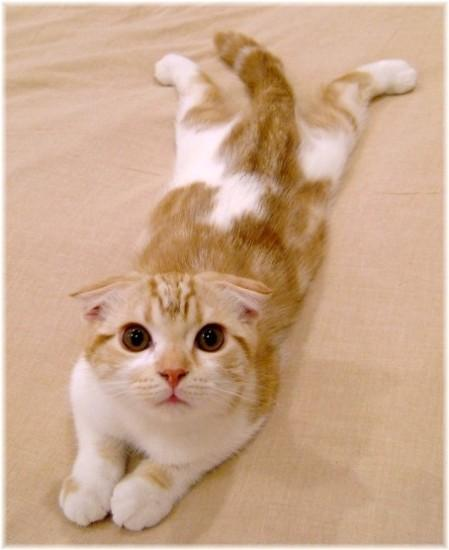
\includegraphics[width=3.5cm]{author.jpg}}},{}]
\end{window}
\daxiaosi
姓名:张 三

性别:男

出生年月:1985~年~00~月~00~日

民族:汉

籍贯:上海市

研究方向:图形图像处理

简历:

\xiaosi
从这里开始写简历

200X.9-200X.7  XX大学XX专业个人简历,从大学起。

200X.9-200X.7  XX大学XX专业个人简历,从大学起。

200X.9-200X.7  XX大学XX专业个人简历,从大学起。

200X.9-200X.7  XX大学XX专业个人简历,从大学起。

%\cleardoublepage

% 授权书
%\chapter*{}
%%\addcontentsline{toc}{chapter}{大连理工大学学位论文版权使用授权书}
%%\addcontentsline{toe}{chapter}{Copyright}
%\renewcommand{\baselinestretch}{1.61}
%\vspace{-0.48cm}
%\authorization
%\cleardoublepage
%
\includepdf{preface/copyright.pdf}
%\cleardoublepage
\end{document}
